% Options for packages loaded elsewhere
\PassOptionsToPackage{unicode}{hyperref}
\PassOptionsToPackage{hyphens}{url}
%
\documentclass[
]{article}
\usepackage{lmodern}
\usepackage{amssymb,amsmath}
\usepackage{ifxetex,ifluatex}
\ifnum 0\ifxetex 1\fi\ifluatex 1\fi=0 % if pdftex
  \usepackage[T1]{fontenc}
  \usepackage[utf8]{inputenc}
  \usepackage{textcomp} % provide euro and other symbols
\else % if luatex or xetex
  \usepackage{unicode-math}
  \defaultfontfeatures{Scale=MatchLowercase}
  \defaultfontfeatures[\rmfamily]{Ligatures=TeX,Scale=1}
\fi
% Use upquote if available, for straight quotes in verbatim environments
\IfFileExists{upquote.sty}{\usepackage{upquote}}{}
\IfFileExists{microtype.sty}{% use microtype if available
  \usepackage[]{microtype}
  \UseMicrotypeSet[protrusion]{basicmath} % disable protrusion for tt fonts
}{}
\makeatletter
\@ifundefined{KOMAClassName}{% if non-KOMA class
  \IfFileExists{parskip.sty}{%
    \usepackage{parskip}
  }{% else
    \setlength{\parindent}{0pt}
    \setlength{\parskip}{6pt plus 2pt minus 1pt}}
}{% if KOMA class
  \KOMAoptions{parskip=half}}
\makeatother
\usepackage{xcolor}
\IfFileExists{xurl.sty}{\usepackage{xurl}}{} % add URL line breaks if available
\IfFileExists{bookmark.sty}{\usepackage{bookmark}}{\usepackage{hyperref}}
\hypersetup{
  pdftitle={Owl Occupancy in Three of El Salvador's Protected Areas from 2003 through 2013},
  pdfauthor={Jane West and Althea Archer},
  hidelinks,
  pdfcreator={LaTeX via pandoc}}
\urlstyle{same} % disable monospaced font for URLs
\usepackage[margin=1in]{geometry}
\usepackage{longtable,booktabs}
% Correct order of tables after \paragraph or \subparagraph
\usepackage{etoolbox}
\makeatletter
\patchcmd\longtable{\par}{\if@noskipsec\mbox{}\fi\par}{}{}
\makeatother
% Allow footnotes in longtable head/foot
\IfFileExists{footnotehyper.sty}{\usepackage{footnotehyper}}{\usepackage{footnote}}
\makesavenoteenv{longtable}
\usepackage{graphicx,grffile}
\makeatletter
\def\maxwidth{\ifdim\Gin@nat@width>\linewidth\linewidth\else\Gin@nat@width\fi}
\def\maxheight{\ifdim\Gin@nat@height>\textheight\textheight\else\Gin@nat@height\fi}
\makeatother
% Scale images if necessary, so that they will not overflow the page
% margins by default, and it is still possible to overwrite the defaults
% using explicit options in \includegraphics[width, height, ...]{}
\setkeys{Gin}{width=\maxwidth,height=\maxheight,keepaspectratio}
% Set default figure placement to htbp
\makeatletter
\def\fps@figure{htbp}
\makeatother
\setlength{\emergencystretch}{3em} % prevent overfull lines
\providecommand{\tightlist}{%
  \setlength{\itemsep}{0pt}\setlength{\parskip}{0pt}}
\setcounter{secnumdepth}{-\maxdimen} % remove section numbering

\title{Owl Occupancy in Three of El Salvador's Protected Areas from 2003
through 2013}
\author{Jane West and Althea Archer}
\date{2/27/2021}

\begin{document}
\maketitle

\hypertarget{abstract}{%
\section{Abstract}\label{abstract}}

\hypertarget{introduction}{%
\section{Introduction}\label{introduction}}

As apex predators, owls are an important bioindicator of ecosystem
health, though much of our understanding comes from temperate systems
(White et al. 2013, Wan et al. 2018, Buechley et al. 2019). In the
tropics, particularly in rain and cloud forests, owl studies are more
difficult than in temperate regions, regardless of potentially denser
populations (König and Weick 1999), and neotropical owls are less
well-studied than their temperate counterparts {[}Buechley:2019{]}.
Further, the neotropics were identified by Buechley et al. (2019) as a
priority area for owl research, based on an extensive literature review
that identified a relative lack of research attention and a high
conservation risk for neotropical owls. As a result, we have limited
understanding of neotropical owls' distribution, ecological
requirements, population dynamics, and reproductive behavior (Clark et
al. 1978, Enríquez et al. 2006, Pérez-Léon et al. 2017, Rangel-Salazar
and Enríquez 2017). This lack of information poses a challenge to
proactive conservation, even as neotropical habitat experiences
tremendous anthropogenic pressure and rapid, unpredictable responses to
climate change (Corlett 2012). In general, while our knowledge about the
status and trends of neotropical owl populations is limited, we do know
that owl abundance and distribution is decreasing in several regions
where species have been added to endangered species lists or have become
locally extirpated (Enríquez et al. 2006).

Like many owl species, neotropical owls are difficult to accurately
census due to their cryptic nature and nocturnal habits. Vocalizations
of crepuscular and cryptic animals such as owls are commonly leveraged
in survey methodology (König and Weick 1999). Owl vocalizations can be
diagnostic and are often considered more practically attainable than
visual identification. Owls vocalize to communicate with the same
species, to threaten or provoke other species, and to delimit territory
(Johnsgard 1988).

Vocalization surveys for nocturnal birds of prey fall generally into two
categories. Spontaneous or ``passive'' surveys involve listening for
animal calls with no prior stimulus, whereas provocation or
``broadcast'' surveys are conducted by listening after a period of
playing a recording of animal vocalizations (e.g., Baumgardt et al.
2019). The inclusion of broadcast calls in auditory surveys can increase
the detection probability of owls, although intra- and inter-species
interactions can play a role whether owls are more likely or less likely
to call in response to a vocalization simulus (Enrı́quez and Salazar
1997, Borges et al. 2004, Flesch and Steidl 2007, Baumgardt et al.
2019).

The objective of our study was to collect occupancy data on El Salvador
owls through time to determine both the population dynamics of
individual owl species and the overall community composition of owls in
three targeted protected areas, El Imposible National Park, Montecristo
National Park, and Nancuchiname Forest. El Salvador is located in the
heart of the Mesoamerican Biodiversity Hotspot (Myers and Mittermeier
2000), and we selected three survey areas in protected landscapes to
represent the breadth of ecosystem diversity across the country. We set
up two routes in each protected area and conducted nighttime foot
surveys using passive listening and broadcast calls during the breeding
season for three weeks during each year from 2003 through 2013.

\hypertarget{methods}{%
\section{Methods}\label{methods}}

\hypertarget{study-area}{%
\subsection{Study area}\label{study-area}}

El Salvador is located on the western side of the Central American
isthmus and is the smallest and most densely populated Central American
country (Central Intelligence Agency 2020). It is bordered by the
Pacific Ocean, Guatemala and Honduras (Fig. 1XXX). Overall, 13.6\% of El
Salvador's 20,720 km\(^2\) of land is forest and 82\% is used for
agricultural purposes (Central Intelligence Agency 2020). We conducted
surveys in three protected natural areas located at different elevations
(high, mid and low elevations) and in different types of forest
vegetation (alluvial, deciduous, semi-deciduous, pine-oak and cloud
forest) that represent a portion of the country's diverse ecosystems
(Fig. 1xxx, Table 1XXX).

El Imposible National Park (NP) was located 119 km southwest of San
Salvador (Fig. 1XXX, Table 1XXX). Its elevation ranged from 250 to 1425
m above sea level (a.s.l.). It was the largest NP in the country,
covering 3792 ha, and its elevation ranged from 250 to 1425 m a.s.l..
The topography of El Imposible was extremely steep and broken, with many
cliffs (Álvarez and Komar 2003). The area contained deciduous and
semi-deciduous forest, secondary growth vegetation on the edges, and
former pasture areas that were reforested with native species in 1997.
We established one survey route (EI-1) in the western portion of El
Imposible in an area of reforestation and at a low elevation and a
second survey route (EI-2) in an area of semi-deciduous forest.

Montecristo NP (1973 ha) was located 125 km northwest of San Salvador
(Fig. 1XXX; Table 1XXX). Its altitude ranged from 730 to 2418 m a.s.l.
(Ministerio de Medio Ambiente y Recursos Naturales 2010). High
elevations of Montecristo contained cloud forest, middle elevations
contained pine/oak forest (with some pine and cypress plantations) and
the lower elevations contained a semi-deciduous tropical forest
(Ministerio de Medio Ambiente y Recursos Naturales 2015a). This NP was
part of the Montecristo Tri-national Protected Area which included
extensive adjoining natural areas in Guatemala and Honduras (Komar
2010). Within Montecristo, we established one survey route (M-1) in a
cloud forest and another (M-2) at a moderate elevation in a pine/oak
forest.

Nancuchiname Forest (797 ha) is a Protected Natural Area located 95 km
southeast of San Salvador in the coastal alluvial plain along the Lempa
River (Fig. 1XXX). Its elevation ranged from sea level to 12 m a.s.l.
The area contained deciduous and semi-deciduous forest, second growth
vegetation, native species reforestation and a dike surrounded by
secondary growth. In Nancuchiname Forest, we established one survey
route (N-1) in alluvial forest along the dike and the other route (N-2)
in a semi-deciduous alluvial forest.

\emph{Table 1XX. Route locations and habitats. Owl surveys were
conducted from 2003 to 2013 in three different protected areas within El
Salvador: El Imposible National Park (EI-1 and EI-2), Montecristo
National Park (M-1 and M-2) and Nancuchiname Forest (N-1 and N-2). }

\begin{longtable}[]{@{}ccccc@{}}
\toprule
\begin{minipage}[b]{0.08\columnwidth}\centering
Route\strut
\end{minipage} & \begin{minipage}[b]{0.15\columnwidth}\centering
Latitude\strut
\end{minipage} & \begin{minipage}[b]{0.15\columnwidth}\centering
Longitude\strut
\end{minipage} & \begin{minipage}[b]{0.13\columnwidth}\centering
Elevation\strut
\end{minipage} & \begin{minipage}[b]{0.35\columnwidth}\centering
Habitat\strut
\end{minipage}\tabularnewline
\midrule
\endhead
\begin{minipage}[t]{0.08\columnwidth}\centering
EI-1\strut
\end{minipage} & \begin{minipage}[t]{0.15\columnwidth}\centering
13xx 50.75'\strut
\end{minipage} & \begin{minipage}[t]{0.15\columnwidth}\centering
89xx 59.74'\strut
\end{minipage} & \begin{minipage}[t]{0.13\columnwidth}\centering
609\strut
\end{minipage} & \begin{minipage}[t]{0.35\columnwidth}\centering
Reforested deciduous forest\strut
\end{minipage}\tabularnewline
\begin{minipage}[t]{0.08\columnwidth}\centering
EI-2\strut
\end{minipage} & \begin{minipage}[t]{0.15\columnwidth}\centering
13xx 51.38'\strut
\end{minipage} & \begin{minipage}[t]{0.15\columnwidth}\centering
89xx 58.24'\strut
\end{minipage} & \begin{minipage}[t]{0.13\columnwidth}\centering
958\strut
\end{minipage} & \begin{minipage}[t]{0.35\columnwidth}\centering
Semi-deciduous forest\strut
\end{minipage}\tabularnewline
\begin{minipage}[t]{0.08\columnwidth}\centering
M-1\strut
\end{minipage} & \begin{minipage}[t]{0.15\columnwidth}\centering
14xx 24.88'\strut
\end{minipage} & \begin{minipage}[t]{0.15\columnwidth}\centering
89xx 21.63'\strut
\end{minipage} & \begin{minipage}[t]{0.13\columnwidth}\centering
2111\strut
\end{minipage} & \begin{minipage}[t]{0.35\columnwidth}\centering
Cloud forest\strut
\end{minipage}\tabularnewline
\begin{minipage}[t]{0.08\columnwidth}\centering
M-2\strut
\end{minipage} & \begin{minipage}[t]{0.15\columnwidth}\centering
14xx 23.19'\strut
\end{minipage} & \begin{minipage}[t]{0.15\columnwidth}\centering
89xx 22.33'\strut
\end{minipage} & \begin{minipage}[t]{0.13\columnwidth}\centering
1755\strut
\end{minipage} & \begin{minipage}[t]{0.35\columnwidth}\centering
Pine/oak forest\strut
\end{minipage}\tabularnewline
\begin{minipage}[t]{0.08\columnwidth}\centering
N-1\strut
\end{minipage} & \begin{minipage}[t]{0.15\columnwidth}\centering
13xx 19.95'\strut
\end{minipage} & \begin{minipage}[t]{0.15\columnwidth}\centering
88xx 43.63'\strut
\end{minipage} & \begin{minipage}[t]{0.13\columnwidth}\centering
3\strut
\end{minipage} & \begin{minipage}[t]{0.35\columnwidth}\centering
Alluvial forest with secondary growth\strut
\end{minipage}\tabularnewline
\begin{minipage}[t]{0.08\columnwidth}\centering
N-2\strut
\end{minipage} & \begin{minipage}[t]{0.15\columnwidth}\centering
13xx 22.03'\strut
\end{minipage} & \begin{minipage}[t]{0.15\columnwidth}\centering
88xx 43.30'\strut
\end{minipage} & \begin{minipage}[t]{0.13\columnwidth}\centering
2\strut
\end{minipage} & \begin{minipage}[t]{0.35\columnwidth}\centering
Alluvial forest\strut
\end{minipage}\tabularnewline
\bottomrule
\end{longtable}

\hypertarget{survey-methods}{%
\subsection{Survey methods}\label{survey-methods}}

We conducted acoustic surveys on foot following the Guidelines for
Nocturnaal Owl Monitoring (Takats et al. 2001), a similar protocol
developed for Costa Rica (Enrı́quez and Rangel-Salazar 2001), and other
raptor research guidelines (Fuller and Mosher 1987). This study's survey
protocol was an extension of previous research completed in the western
half of El Imposible NP (West 1988). We created six 2-km long survey
routes (transects) that each included 10 permanent survey stations set
at 200 m intervals. Two routes were established in each protected area
(Table 1xxx).

Surveys began at local twilight and took approximately five hours to
complete. At each station, we measured and recorded environmental
conditions (Brunton Sherpa, Brunton Incorporated) including temperature,
precipitation, cloud cover, fog cover, wind speed, barometric pressure,
moon phase, and noise level. The acoustic survey then began with passive
listening for two minutes, followed by a three-minute broadcast call,
and ending with seven minutes of silent listening. We recorded local owl
vocalizations and used them for broadcast calls whenever possible. If an
owl vocalized during broadcast playback, we stopped the broadcast and
recorded the owl's vocalization. When we detected an owl, we noted its
location and bearing relative to the station, and we tracked when the
same owl was identified at consecutive stations.

The broadcast calls varied between routes, but were consistent at each
route and station across years. Specifically, we broadcast the
vocalizations of Pacific Screech-Owls (\emph{Megascops cooperi}),
Mottled Owls (\emph{Ciccaba virgata}), Crested Owls (\emph{Lophostrix
cristata}), Black-and-white Owls (\emph{C. nigrolineata}), Spectacled
Owls (\emph{Pulsatrix perspicillata}), Pacific Screech-Owls, Mottled
Owls, Crested Owls, Black-and-white Owls, and Spectacled Owls at
stations 1 through 10, respectively, in all routes in El Imposible NP
(EI-1 and EI-2) and Nancuchiname Forest (N-1 and N-2). We broadcast the
vocalizations of Whiskered Owls (\emph{M. trichopsis}), Mottled Owls,
Fulvous Owls (\emph{Strix fulvescens}), Stygian Owls (\emph{Asio
stygius}), Great Horned Owls (\emph{Bubo virginianus}), Whiskered Owls,
Mottled Owls, Fulvous Owls, Stygian Owls, and Great Horned Owls at
stations 1 through 10, respectively, in both routes of Montecristo NP
(M-1 and M-2).

Surveys were repeated at each route up to three times a year from 2003
through 2013, depending on site access and weather. We did not conduct
any surveys in 2006. We georeferenced the owl detections for each survey
and route to eliminate double counting of individual owl observations.

\emph{Table 2XX. Species detection records by route. Owl surveys were
conducted from 2003 to 2013 in three different protected areas within El
Salvador, although specific survey years varied by route.}

\begin{longtable}[]{@{}ccccccc@{}}
\toprule
\begin{minipage}[b]{0.31\columnwidth}\centering
Name\strut
\end{minipage} & \begin{minipage}[b]{0.08\columnwidth}\centering
EI-1\strut
\end{minipage} & \begin{minipage}[b]{0.08\columnwidth}\centering
EI-2\strut
\end{minipage} & \begin{minipage}[b]{0.07\columnwidth}\centering
M-1\strut
\end{minipage} & \begin{minipage}[b]{0.07\columnwidth}\centering
M-2\strut
\end{minipage} & \begin{minipage}[b]{0.07\columnwidth}\centering
N-1\strut
\end{minipage} & \begin{minipage}[b]{0.07\columnwidth}\centering
N-2\strut
\end{minipage}\tabularnewline
\midrule
\endhead
\begin{minipage}[t]{0.31\columnwidth}\centering
Barn Owl\strut
\end{minipage} & \begin{minipage}[t]{0.08\columnwidth}\centering
0\strut
\end{minipage} & \begin{minipage}[t]{0.08\columnwidth}\centering
0\strut
\end{minipage} & \begin{minipage}[t]{0.07\columnwidth}\centering
0\strut
\end{minipage} & \begin{minipage}[t]{0.07\columnwidth}\centering
0\strut
\end{minipage} & \begin{minipage}[t]{0.07\columnwidth}\centering
8\strut
\end{minipage} & \begin{minipage}[t]{0.07\columnwidth}\centering
2\strut
\end{minipage}\tabularnewline
\begin{minipage}[t]{0.31\columnwidth}\centering
(Tyto alba)\strut
\end{minipage} & \begin{minipage}[t]{0.08\columnwidth}\centering
\strut
\end{minipage} & \begin{minipage}[t]{0.08\columnwidth}\centering
\strut
\end{minipage} & \begin{minipage}[t]{0.07\columnwidth}\centering
\strut
\end{minipage} & \begin{minipage}[t]{0.07\columnwidth}\centering
\strut
\end{minipage} & \begin{minipage}[t]{0.07\columnwidth}\centering
\strut
\end{minipage} & \begin{minipage}[t]{0.07\columnwidth}\centering
\strut
\end{minipage}\tabularnewline
\begin{minipage}[t]{0.31\columnwidth}\centering
Whiskered Screech-Owl\strut
\end{minipage} & \begin{minipage}[t]{0.08\columnwidth}\centering
0\strut
\end{minipage} & \begin{minipage}[t]{0.08\columnwidth}\centering
0\strut
\end{minipage} & \begin{minipage}[t]{0.07\columnwidth}\centering
0\strut
\end{minipage} & \begin{minipage}[t]{0.07\columnwidth}\centering
2\strut
\end{minipage} & \begin{minipage}[t]{0.07\columnwidth}\centering
0\strut
\end{minipage} & \begin{minipage}[t]{0.07\columnwidth}\centering
0\strut
\end{minipage}\tabularnewline
\begin{minipage}[t]{0.31\columnwidth}\centering
(Megascops trichopsis)\strut
\end{minipage} & \begin{minipage}[t]{0.08\columnwidth}\centering
\strut
\end{minipage} & \begin{minipage}[t]{0.08\columnwidth}\centering
\strut
\end{minipage} & \begin{minipage}[t]{0.07\columnwidth}\centering
\strut
\end{minipage} & \begin{minipage}[t]{0.07\columnwidth}\centering
\strut
\end{minipage} & \begin{minipage}[t]{0.07\columnwidth}\centering
\strut
\end{minipage} & \begin{minipage}[t]{0.07\columnwidth}\centering
\strut
\end{minipage}\tabularnewline
\begin{minipage}[t]{0.31\columnwidth}\centering
Pacific Screech-Owl\strut
\end{minipage} & \begin{minipage}[t]{0.08\columnwidth}\centering
11\strut
\end{minipage} & \begin{minipage}[t]{0.08\columnwidth}\centering
1\strut
\end{minipage} & \begin{minipage}[t]{0.07\columnwidth}\centering
0\strut
\end{minipage} & \begin{minipage}[t]{0.07\columnwidth}\centering
0\strut
\end{minipage} & \begin{minipage}[t]{0.07\columnwidth}\centering
6\strut
\end{minipage} & \begin{minipage}[t]{0.07\columnwidth}\centering
9\strut
\end{minipage}\tabularnewline
\begin{minipage}[t]{0.31\columnwidth}\centering
(Megascops cooperi)\strut
\end{minipage} & \begin{minipage}[t]{0.08\columnwidth}\centering
\strut
\end{minipage} & \begin{minipage}[t]{0.08\columnwidth}\centering
\strut
\end{minipage} & \begin{minipage}[t]{0.07\columnwidth}\centering
\strut
\end{minipage} & \begin{minipage}[t]{0.07\columnwidth}\centering
\strut
\end{minipage} & \begin{minipage}[t]{0.07\columnwidth}\centering
\strut
\end{minipage} & \begin{minipage}[t]{0.07\columnwidth}\centering
\strut
\end{minipage}\tabularnewline
\begin{minipage}[t]{0.31\columnwidth}\centering
Crested Owl\strut
\end{minipage} & \begin{minipage}[t]{0.08\columnwidth}\centering
0\strut
\end{minipage} & \begin{minipage}[t]{0.08\columnwidth}\centering
0\strut
\end{minipage} & \begin{minipage}[t]{0.07\columnwidth}\centering
0\strut
\end{minipage} & \begin{minipage}[t]{0.07\columnwidth}\centering
0\strut
\end{minipage} & \begin{minipage}[t]{0.07\columnwidth}\centering
0\strut
\end{minipage} & \begin{minipage}[t]{0.07\columnwidth}\centering
0\strut
\end{minipage}\tabularnewline
\begin{minipage}[t]{0.31\columnwidth}\centering
(Lophostrix cristata)\strut
\end{minipage} & \begin{minipage}[t]{0.08\columnwidth}\centering
\strut
\end{minipage} & \begin{minipage}[t]{0.08\columnwidth}\centering
\strut
\end{minipage} & \begin{minipage}[t]{0.07\columnwidth}\centering
\strut
\end{minipage} & \begin{minipage}[t]{0.07\columnwidth}\centering
\strut
\end{minipage} & \begin{minipage}[t]{0.07\columnwidth}\centering
\strut
\end{minipage} & \begin{minipage}[t]{0.07\columnwidth}\centering
\strut
\end{minipage}\tabularnewline
\begin{minipage}[t]{0.31\columnwidth}\centering
Spectacled Owl**\strut
\end{minipage} & \begin{minipage}[t]{0.08\columnwidth}\centering
1\strut
\end{minipage} & \begin{minipage}[t]{0.08\columnwidth}\centering
1\strut
\end{minipage} & \begin{minipage}[t]{0.07\columnwidth}\centering
0\strut
\end{minipage} & \begin{minipage}[t]{0.07\columnwidth}\centering
1\strut
\end{minipage} & \begin{minipage}[t]{0.07\columnwidth}\centering
59\strut
\end{minipage} & \begin{minipage}[t]{0.07\columnwidth}\centering
75\strut
\end{minipage}\tabularnewline
\begin{minipage}[t]{0.31\columnwidth}\centering
(Pulsatrix perspicillata)\strut
\end{minipage} & \begin{minipage}[t]{0.08\columnwidth}\centering
\strut
\end{minipage} & \begin{minipage}[t]{0.08\columnwidth}\centering
\strut
\end{minipage} & \begin{minipage}[t]{0.07\columnwidth}\centering
\strut
\end{minipage} & \begin{minipage}[t]{0.07\columnwidth}\centering
\strut
\end{minipage} & \begin{minipage}[t]{0.07\columnwidth}\centering
\strut
\end{minipage} & \begin{minipage}[t]{0.07\columnwidth}\centering
\strut
\end{minipage}\tabularnewline
\begin{minipage}[t]{0.31\columnwidth}\centering
Great Horned Owl\strut
\end{minipage} & \begin{minipage}[t]{0.08\columnwidth}\centering
0\strut
\end{minipage} & \begin{minipage}[t]{0.08\columnwidth}\centering
0\strut
\end{minipage} & \begin{minipage}[t]{0.07\columnwidth}\centering
3\strut
\end{minipage} & \begin{minipage}[t]{0.07\columnwidth}\centering
0\strut
\end{minipage} & \begin{minipage}[t]{0.07\columnwidth}\centering
0\strut
\end{minipage} & \begin{minipage}[t]{0.07\columnwidth}\centering
0\strut
\end{minipage}\tabularnewline
\begin{minipage}[t]{0.31\columnwidth}\centering
(Bubo virginianus)\strut
\end{minipage} & \begin{minipage}[t]{0.08\columnwidth}\centering
\strut
\end{minipage} & \begin{minipage}[t]{0.08\columnwidth}\centering
\strut
\end{minipage} & \begin{minipage}[t]{0.07\columnwidth}\centering
\strut
\end{minipage} & \begin{minipage}[t]{0.07\columnwidth}\centering
\strut
\end{minipage} & \begin{minipage}[t]{0.07\columnwidth}\centering
\strut
\end{minipage} & \begin{minipage}[t]{0.07\columnwidth}\centering
\strut
\end{minipage}\tabularnewline
\begin{minipage}[t]{0.31\columnwidth}\centering
Ferruginous Pygmy-Owl\strut
\end{minipage} & \begin{minipage}[t]{0.08\columnwidth}\centering
4\strut
\end{minipage} & \begin{minipage}[t]{0.08\columnwidth}\centering
0\strut
\end{minipage} & \begin{minipage}[t]{0.07\columnwidth}\centering
0\strut
\end{minipage} & \begin{minipage}[t]{0.07\columnwidth}\centering
0\strut
\end{minipage} & \begin{minipage}[t]{0.07\columnwidth}\centering
82\strut
\end{minipage} & \begin{minipage}[t]{0.07\columnwidth}\centering
98\strut
\end{minipage}\tabularnewline
\begin{minipage}[t]{0.31\columnwidth}\centering
(Glaucidium brasilianum)\strut
\end{minipage} & \begin{minipage}[t]{0.08\columnwidth}\centering
\strut
\end{minipage} & \begin{minipage}[t]{0.08\columnwidth}\centering
\strut
\end{minipage} & \begin{minipage}[t]{0.07\columnwidth}\centering
\strut
\end{minipage} & \begin{minipage}[t]{0.07\columnwidth}\centering
\strut
\end{minipage} & \begin{minipage}[t]{0.07\columnwidth}\centering
\strut
\end{minipage} & \begin{minipage}[t]{0.07\columnwidth}\centering
\strut
\end{minipage}\tabularnewline
\begin{minipage}[t]{0.31\columnwidth}\centering
Burrowing Owl\strut
\end{minipage} & \begin{minipage}[t]{0.08\columnwidth}\centering
0\strut
\end{minipage} & \begin{minipage}[t]{0.08\columnwidth}\centering
0\strut
\end{minipage} & \begin{minipage}[t]{0.07\columnwidth}\centering
0\strut
\end{minipage} & \begin{minipage}[t]{0.07\columnwidth}\centering
0\strut
\end{minipage} & \begin{minipage}[t]{0.07\columnwidth}\centering
0\strut
\end{minipage} & \begin{minipage}[t]{0.07\columnwidth}\centering
0\strut
\end{minipage}\tabularnewline
\begin{minipage}[t]{0.31\columnwidth}\centering
(Athene cunicularia)\strut
\end{minipage} & \begin{minipage}[t]{0.08\columnwidth}\centering
\strut
\end{minipage} & \begin{minipage}[t]{0.08\columnwidth}\centering
\strut
\end{minipage} & \begin{minipage}[t]{0.07\columnwidth}\centering
\strut
\end{minipage} & \begin{minipage}[t]{0.07\columnwidth}\centering
\strut
\end{minipage} & \begin{minipage}[t]{0.07\columnwidth}\centering
\strut
\end{minipage} & \begin{minipage}[t]{0.07\columnwidth}\centering
\strut
\end{minipage}\tabularnewline
\begin{minipage}[t]{0.31\columnwidth}\centering
Mottled Owl\strut
\end{minipage} & \begin{minipage}[t]{0.08\columnwidth}\centering
214\strut
\end{minipage} & \begin{minipage}[t]{0.08\columnwidth}\centering
117\strut
\end{minipage} & \begin{minipage}[t]{0.07\columnwidth}\centering
1\strut
\end{minipage} & \begin{minipage}[t]{0.07\columnwidth}\centering
22\strut
\end{minipage} & \begin{minipage}[t]{0.07\columnwidth}\centering
62\strut
\end{minipage} & \begin{minipage}[t]{0.07\columnwidth}\centering
114\strut
\end{minipage}\tabularnewline
\begin{minipage}[t]{0.31\columnwidth}\centering
(Ciccaba virgata)\strut
\end{minipage} & \begin{minipage}[t]{0.08\columnwidth}\centering
\strut
\end{minipage} & \begin{minipage}[t]{0.08\columnwidth}\centering
\strut
\end{minipage} & \begin{minipage}[t]{0.07\columnwidth}\centering
\strut
\end{minipage} & \begin{minipage}[t]{0.07\columnwidth}\centering
\strut
\end{minipage} & \begin{minipage}[t]{0.07\columnwidth}\centering
\strut
\end{minipage} & \begin{minipage}[t]{0.07\columnwidth}\centering
\strut
\end{minipage}\tabularnewline
\begin{minipage}[t]{0.31\columnwidth}\centering
Black-and-white Owl**\strut
\end{minipage} & \begin{minipage}[t]{0.08\columnwidth}\centering
0\strut
\end{minipage} & \begin{minipage}[t]{0.08\columnwidth}\centering
0\strut
\end{minipage} & \begin{minipage}[t]{0.07\columnwidth}\centering
0\strut
\end{minipage} & \begin{minipage}[t]{0.07\columnwidth}\centering
0\strut
\end{minipage} & \begin{minipage}[t]{0.07\columnwidth}\centering
0\strut
\end{minipage} & \begin{minipage}[t]{0.07\columnwidth}\centering
0\strut
\end{minipage}\tabularnewline
\begin{minipage}[t]{0.31\columnwidth}\centering
(Ciccaba nigrolineata)\strut
\end{minipage} & \begin{minipage}[t]{0.08\columnwidth}\centering
\strut
\end{minipage} & \begin{minipage}[t]{0.08\columnwidth}\centering
\strut
\end{minipage} & \begin{minipage}[t]{0.07\columnwidth}\centering
\strut
\end{minipage} & \begin{minipage}[t]{0.07\columnwidth}\centering
\strut
\end{minipage} & \begin{minipage}[t]{0.07\columnwidth}\centering
\strut
\end{minipage} & \begin{minipage}[t]{0.07\columnwidth}\centering
\strut
\end{minipage}\tabularnewline
\begin{minipage}[t]{0.31\columnwidth}\centering
Fulvous Owl*\strut
\end{minipage} & \begin{minipage}[t]{0.08\columnwidth}\centering
0\strut
\end{minipage} & \begin{minipage}[t]{0.08\columnwidth}\centering
0\strut
\end{minipage} & \begin{minipage}[t]{0.07\columnwidth}\centering
17\strut
\end{minipage} & \begin{minipage}[t]{0.07\columnwidth}\centering
0\strut
\end{minipage} & \begin{minipage}[t]{0.07\columnwidth}\centering
0\strut
\end{minipage} & \begin{minipage}[t]{0.07\columnwidth}\centering
0\strut
\end{minipage}\tabularnewline
\begin{minipage}[t]{0.31\columnwidth}\centering
(Strix fulvescens)\strut
\end{minipage} & \begin{minipage}[t]{0.08\columnwidth}\centering
\strut
\end{minipage} & \begin{minipage}[t]{0.08\columnwidth}\centering
\strut
\end{minipage} & \begin{minipage}[t]{0.07\columnwidth}\centering
\strut
\end{minipage} & \begin{minipage}[t]{0.07\columnwidth}\centering
\strut
\end{minipage} & \begin{minipage}[t]{0.07\columnwidth}\centering
\strut
\end{minipage} & \begin{minipage}[t]{0.07\columnwidth}\centering
\strut
\end{minipage}\tabularnewline
\begin{minipage}[t]{0.31\columnwidth}\centering
c.f. Stygian Owl\strut
\end{minipage} & \begin{minipage}[t]{0.08\columnwidth}\centering
0\strut
\end{minipage} & \begin{minipage}[t]{0.08\columnwidth}\centering
0\strut
\end{minipage} & \begin{minipage}[t]{0.07\columnwidth}\centering
0\strut
\end{minipage} & \begin{minipage}[t]{0.07\columnwidth}\centering
1\strut
\end{minipage} & \begin{minipage}[t]{0.07\columnwidth}\centering
0\strut
\end{minipage} & \begin{minipage}[t]{0.07\columnwidth}\centering
0\strut
\end{minipage}\tabularnewline
\begin{minipage}[t]{0.31\columnwidth}\centering
(Asio stygius)\strut
\end{minipage} & \begin{minipage}[t]{0.08\columnwidth}\centering
\strut
\end{minipage} & \begin{minipage}[t]{0.08\columnwidth}\centering
\strut
\end{minipage} & \begin{minipage}[t]{0.07\columnwidth}\centering
\strut
\end{minipage} & \begin{minipage}[t]{0.07\columnwidth}\centering
\strut
\end{minipage} & \begin{minipage}[t]{0.07\columnwidth}\centering
\strut
\end{minipage} & \begin{minipage}[t]{0.07\columnwidth}\centering
\strut
\end{minipage}\tabularnewline
\begin{minipage}[t]{0.31\columnwidth}\centering
Striped Owl\strut
\end{minipage} & \begin{minipage}[t]{0.08\columnwidth}\centering
0\strut
\end{minipage} & \begin{minipage}[t]{0.08\columnwidth}\centering
0\strut
\end{minipage} & \begin{minipage}[t]{0.07\columnwidth}\centering
0\strut
\end{minipage} & \begin{minipage}[t]{0.07\columnwidth}\centering
0\strut
\end{minipage} & \begin{minipage}[t]{0.07\columnwidth}\centering
0\strut
\end{minipage} & \begin{minipage}[t]{0.07\columnwidth}\centering
0\strut
\end{minipage}\tabularnewline
\begin{minipage}[t]{0.31\columnwidth}\centering
(Pseudoscops clamator)\strut
\end{minipage} & \begin{minipage}[t]{0.08\columnwidth}\centering
\strut
\end{minipage} & \begin{minipage}[t]{0.08\columnwidth}\centering
\strut
\end{minipage} & \begin{minipage}[t]{0.07\columnwidth}\centering
\strut
\end{minipage} & \begin{minipage}[t]{0.07\columnwidth}\centering
\strut
\end{minipage} & \begin{minipage}[t]{0.07\columnwidth}\centering
\strut
\end{minipage} & \begin{minipage}[t]{0.07\columnwidth}\centering
\strut
\end{minipage}\tabularnewline
\begin{minipage}[t]{0.31\columnwidth}\centering
Unspotted Saw-whet Owl\strut
\end{minipage} & \begin{minipage}[t]{0.08\columnwidth}\centering
0\strut
\end{minipage} & \begin{minipage}[t]{0.08\columnwidth}\centering
0\strut
\end{minipage} & \begin{minipage}[t]{0.07\columnwidth}\centering
0\strut
\end{minipage} & \begin{minipage}[t]{0.07\columnwidth}\centering
0\strut
\end{minipage} & \begin{minipage}[t]{0.07\columnwidth}\centering
0\strut
\end{minipage} & \begin{minipage}[t]{0.07\columnwidth}\centering
0\strut
\end{minipage}\tabularnewline
\begin{minipage}[t]{0.31\columnwidth}\centering
(Aegolius ridgwayi)\strut
\end{minipage} & \begin{minipage}[t]{0.08\columnwidth}\centering
\strut
\end{minipage} & \begin{minipage}[t]{0.08\columnwidth}\centering
\strut
\end{minipage} & \begin{minipage}[t]{0.07\columnwidth}\centering
\strut
\end{minipage} & \begin{minipage}[t]{0.07\columnwidth}\centering
\strut
\end{minipage} & \begin{minipage}[t]{0.07\columnwidth}\centering
\strut
\end{minipage} & \begin{minipage}[t]{0.07\columnwidth}\centering
\strut
\end{minipage}\tabularnewline
\bottomrule
\end{longtable}

\emph{Note: ** = Endangered and * = Threatened (Ministerio de Medio
Ambiente y Recursos Naturales 2015b)}

\hypertarget{single-species-occupancy-model-framework}{%
\subsection{Single-species occupancy model
framework}\label{single-species-occupancy-model-framework}}

We modeled occupancy within each route, year, and survey assuming that
the probability of occupancy would be closed across surveys of a given
route in a given year. In other words, for any single species of owl, we
assumed that the probability of a route being occupied would not change
between surveys within a year but could vary between years. Let:

\[
\begin{aligned}
t  &=  \text{the year each survey was conducted (}t = 1,2,\ldots,11)\text{ representing 2003-2013}\\
h  &=  \text{the individual route (}h = 1,2,\ldots,6)\text{ representing EI-1, EI-2, M-1, M-2, N-1, N-2}\\
i  &=  \text{the individual surveys conducted in each year and route (}i = 1,2,3)\\
j  &=  \text{the individual stations along each route (}j = 1,2,\ldots,10)\\
k  &=  \text{the broadcast call species (}k = 1,2,\ldots,10)\\
z_{t,h,i} &= \text{a random variable equal to 1 when a survey route was occupied and 0 otherwise}\\
y_{t,h,i,j,k} &= \text{a random variable equal to 1 when an owl was detected and 0 otherwise}
\end{aligned}
\]

We assumed that occupancy in each individual survey (\(z_{t,h,i}\)) was
the outcome of Bernoulli trials with a probability of occupancy,
\(\psi_{t,h}\), which we allowed to vary by year and route:

\[
z_{t,h,i} \sim \text{Bernoulli}(\psi_{t,h})
\]

\[
\psi_{t,h} \sim \text{Beta}(a^\psi_{t,h},b^\psi_{t,h})
\] with hyperpriors for \(a^\psi_{t,h}\) and \(b^\psi_{t,h}\) such that
the expected value of \(\psi_{t,h} = \mu^\psi_{t,h}\):

\[
\begin{aligned}
\text{E}[\psi_{t,h}] &= \mu^\psi_{t,h} = a^\psi_{t,h}/(a^\psi_{t,h}+b^\psi_{t,h})\\
\rho^\psi_{t,h} &= a^\psi_{t,h}+b^\psi_{t,h}\\
\text{logit}(\mu^\psi_{t,h}) &\sim \text{N}(0, 2.25)\\
\ln(\rho^\psi_{t,h}) &\sim \text{N}(5,1)\text{, truncated to 0.01,10}\\
\end{aligned}
\]

We assumed that detecting an owl depended on an owl being present during
that survey (\(z_{t,h,i} = 1\)) and the probability of detection,
\(p_{t,h,i,j,k}\), which was related to the species-specific broadcast
call (\(k\)):

\[
y_{t,h,i,j,k} \sim \text{Bernoulli}(z_{t,h,i}*p_{t,h,i,j,k})
\]

where, generally, \(\text{logit}(p_{t,h,i,j,k}) = \beta_kX_k\), or more
specifically:

\[
\begin{aligned}
\text{logit}(p_{t,h,i,j,k}) &= \beta_\text{Pre-broadcast}X_\text{Pre-broadcast} + \\
&= \beta_\text{Mottled}X_\text{Mottled}+\\
&= \beta_\text{Pacific}X_\text{Pacific}+\\
&= \beta_\text{Crested}X_\text{Crested}+\\
&= \beta_\text{Black and White}X_\text{Black and White}+\\
&= \beta_\text{Spectacled}X_\text{Spectacled}+\\
&= \beta_\text{Whiskered}X_\text{Whiskered}+\\
&= \beta_\text{Guat Barred}X_\text{Guat Barred}+\\
&= \beta_\text{Stygian}X_\text{Stygian}+\\
&= \beta_\text{Great Horned}X_\text{Great Horned}\\
\end{aligned}
\]

This model provided a consistent probability of detection for all
surveys in the first two minutes of each observation period, before the
broadcast call was played (\(k = \text{Pre-broadcast}\)). Then, the
probability of detection for each post-broadcast time period depended
which call had been played. This allowed species-specific behavior in
response to the different broadcast calls (Baumgardt et al. 2019). We
used means parameterization for the logistic regression model such that
the coefficients were interpretable as the effect of that specific
broadcast call \(k\) (including the pre-broadcast time frame). The
priors for every logistic model coefficient \(\beta_k\) were chosen to
be near uniform as recommended in Gelman et al. (2008):
\(\beta_k \sim \text{Cauchy}(\text{precision} = 0.16)\).

\hypertarget{richness-model-framework}{%
\subsection{Richness model framework}\label{richness-model-framework}}

To model species richness at each route in each year, we assumed that
there were 14 possible species present in El Salvador. This included the
9 species observed during our surveys and an additional 5 species that
we never observed (Table 2XX). This upper limit to expected species
richness related directly to the 13 species known to inhabit El Salvador
(Dickey and van Rossem 1938) plus one species we identified (c.f.
Stygian owl), which was previously undocumented in El Salvador. We thus
augmented our owl detection data with 5 additional potential species
with all-zero detection records (Royle 2007).

For each species \(s\) (where \(s = 1,2, \ldots,15\)), \(w_{h,s}\) was a
binary indicator of whether that owl species was present in each route
based on the probability of species presence in that route, \(\Omega_h\)
(Broms et al. 2016):

\[
w_{h,s} \sim \text{Bernoulli}(\Omega_h)
\] We used prior distributions for \(\Omega_h\):
\(\Omega_h \sim \text{Beta}(0.001, 1)\) (Broms et al. 2016,
Guillera-Arroita et al. 2019).

In the richness model, the presence of an owl species in any year,
route, and survey, \(z_{t,h,i,s}\), was conditional on the probability
of occupancy for that route, year, and species \(\psi_{t,h,s}\)
\emph{and} that species belonging to that route's community that year
(\(w_{h,s}\)):

\[
z_{t,h,i,s} \sim \text{Bernoulli}(w_{h,s}*\psi_{t,h,s})
\]

To share information about occupancy amongst species, we incorporated
random effects into the parameterization of \(\psi_{t,h,s}\):

\[
\begin{aligned}
\psi_{t,h,s} &\sim \text{Beta}(a^\psi_{t,h,s},b^\psi_{t,h,s})\\ 
a^\psi_{t,h,s} &= \mu^\psi_{t,h}\rho^\psi\\
b^\psi_{t,h,s} &= \rho^\psi - \mu^\psi_{t,h}\rho^\psi\\
\text{logit}(\mu^\psi_{t,h}) &\sim N(0,2.25)\\
\ln(\rho^\psi) &\sim N(5,1)\text{, truncated to (0.01,10)}\\
\end{aligned}
\]

This parameterization allowed us to borrow strength across species in
determining the mean probability of occupancy (\(\mu^\psi_{t,h}\)) for
each route and year (Guillera-Arroita et al. 2019).

Richness of each route was conditional on each species' presence and was
estimated as the sum of owl species present in that route:

\[
\text{Richness}_{h} = \sum_{s=1}^{15} w_{h,s} 
\]

We also estimated year-to-year richness (\(\text{Richness}^*_{t,h}\)) by
route by adding up the number of unique species that were present in
each route, year, and survey. We first determined if a species was
present in any of that route and year's set of surveys with a
species-specific binary indicator \(\vartheta_{t,h,s}\) where
\(\vartheta_{t,h,s} = 1\) if \(z_{t,h,i,s} = 1\) in any of that route's
surveys \(i\) that year. Then, we summed up the number of species
present in each year and route: \[
\text{Richness}^*_{t,h} = \sum_{s=1}^{15} \vartheta_{t,h,s} 
\]

Consistent with our approach for the occupancy models, we assumed that
detecting an owl depended on an individual of that species being present
during that survey (\(z_{t,h,i,s} = 1\)) and the species-specific
probability of detection \(p_{t,h,i,j,k,s}\), which was related to the
broadcast call:

\[
y_{t,h,i,j,k,s} \sim \text{Bernoulli}(z_{t,h,i,s}*p_{t,h,i,j,k,s})
\]

where generally \(\text{logit}(p_{t,h,i,j,k,s}) = \beta_kX_k\) for each
broadcast call \(k\) as described above. The coefficients of the
detection model were thus assumed to be consistent for all owl species,
which allowed us to borrow information about the detection process for
undetected owl species from those that were detected.

\hypertarget{model-implementation}{%
\subsubsection{Model implementation}\label{model-implementation}}

We used the R2jags package in R (R Development Core Team 2014) (Plummer
2013) to implement the Bayesian models. We verified that R-hats were
lower than 1.3 and visually inspected traceplots to verify that chains
mixed well (Supplemental information S1-3xx).

We applied the single-species occupancy model for three owl species that
had sufficient positive detections for analysis: Mottled Owl, Spectacled
Owl, and Ferruginous Pygmy-Owl (Table 2XX). Based on our understanding
of owl ecology, we assumed that Spectacled and Ferruginous Pygmy owls
would not occupy route M-1 in Montecristo, so we removed M-1 from those
species' occupancy analyses. For all three of the single-species
occupancy models, we ran 3 chains for 10,000 iterations and 1000
iterations discarded as burn-in, for a total of 27,000 iterations
comprising the posterior distributions for each model parameter. Initial
values for \(z_{t,h,i}\) were equivalent to one if an owl was detected
in that survey \(i\) and otherwise zero.

To implement the richness model, we ran 3 chains for 20,000 iterations
with 2000 iterations discarded as burn-in and a thinning rate of 2, for
a total of 27,000 iterations comprising the posterior distributions for
each model parameter. Initial values for \(z_{t,h,i,s}\) were equivalent
to one if that species of owl was detected in that survey and otherwise
zero. Similarly, initial values for whether a species belonged to a
route's community (\(w_{h,s}\)) were equivalent to one if that species
of owl was ever detected in that route and otherwise zero.

\hypertarget{results}{%
\section{Results}\label{results}}

A total of 86 surveys were conducted between March and May from 2003
through 2005 and 2007 through 2013. No surveys were conducted in 2006.

We detected nine species of owls during our surveys: Barn Owl, Whiskered
Screech-Owl, Pacific Screech-Owl, Spectacled Owl, Great Horned Owl,
Ferruginous Pygmy-Owl, Mottled Owl, Fulvous Owl, and c.f. Stygian Owl
(Table 2xXX). We identified Whiskered Screech-Owls in Montecristo NP,
which had previously been undocumented in that protected area. We also
identified a c.f. Stygian Owl in Montecristo NP, which was a species not
previously documented in the entire country of El Salvador. The c.f.
Stygian Owl requires further investigation to determine true presence of
that owl in El Salvador.

\hypertarget{single-species-occupancy-model-results}{%
\subsection{Single-species occupancy model
results}\label{single-species-occupancy-model-results}}

Mottled Owls, Spectacled Owls, and Ferruginous Pygmy-Owls had 542, 137,
and 187 positive detections over the 11 year period, respectively (Table
2XX). No other owl species had enough detections to analyze
species-specific occupancy (Table 2XX). Averaged across years, we found
that the probability of occupancy was somewhat higher for Mottled Owls
than for Ferruginous Pygmy-owls or Spectacled Owls in both routes of El
Imposible and in M-2 route of Montecristo (Fig. 1X). Occupancy
probabilities were relatively high across all three species for both
routes of Nancuchiname (Fig. 2XX). We found that the probability of
occupancy for Mottled Owls was relatively consistent across time in both
El Imposible routes and in N-2 (Fig. 3XX), but that it seemed to
increase in the last approximately 6 years in M-2 and N-1 (Fig. 3XX).
The probability of occupancy in M-1 seemed to have decreased through
time for Mottled Owls (Fig. 3XX).

For routes EI-1, EI-2, and M-2, the probability of occupancy for
Ferruginous Pygmy-owls and Spectacled Owls stayed relatively low across
time other than a higher probability of occupancy for Ferruginous
Pygmy-owl in EI-1 in the early years of the surveys (Fig. 3XX). The
probability of occupancy for Ferruginous Pygmy-owls was relatively high
in both routes of Nancuchaname except in 2008 and 2009 (Fig. 3XX), and
the probability of occupancy for the Spectacled Owl fluctuated slightly
from year to year in the Nancuchaname routes (Fig. 3XX).

\hypertarget{richness-model-results}{%
\subsection{Richness model results}\label{richness-model-results}}

Our estimates of each route's community richness
(\(\text{Richness}_{h}\)) and 90\% credible intervals were 4 (4,4), 3
(3,3), 3 (3,4), 4 (4,5), 5 (5,5), and 5 (5,5) for EI-1, EI-2, M-1, M-2,
N-1, and N-2, respectively. These median values were equivalent to the
number of species detected in each route (Table 2XX), indicating that
the probability of occupancy for undetected species was low and no
additional species were predicted to be present in a route's community,
other than those that were detected.

When analyzed by year and route, median species richness
(\(\text{Richness}^*_{t,h}\)) varied from 0 to 5 (Fig. 4XXX). At most,
the median species richness was one species higher than the number of
species detected at any single route and year; however, the 90\%
credible intervals of richness added up to 4 new undetected species
(e.g., in M-2 during 2004 where we detected zero species (Fig. 4XXX).

\hypertarget{detection-results}{%
\subsection{Detection results}\label{detection-results}}

Including all detected species in one richness model increased the
precision of the estimates of the effect of broadcast calls on detection
probability (i.e., compare All Species with individual occupancy results
in Fig. 5XXX). When incorporating all owl species, broadcasting calls
from Mottled Owls, Pacific Screech-owls, Crested Owls, Black-and-white
Owls, and Spectacled Owls increased detection probability; whereas
broadcasting the Great Horned Owl calls decreased detection (Fig. 5XXX).

The probability of detection when analyzed with single-species occupancy
models varied little during the timeframe before broadcast recordings
were played (Pre-broadcast); however, the probability of detecting owls
after broadcast calls were played varied by call and between Mottled
Owls, Ferruginous Pygmy-owls, and Spectacled Owls (Fig. 5XX). The
probability of detecting Mottled Owls increased after broadcasting
Mottled Owl, Pacific Screech-owl, Crested Owl, Black-and-white Owl, or
Spectacled Owl calls. The probability of detecting Ferruginous
Pygmy-owls increased after broadcasting Mottled Owl and Pacific Owl
calls, and the probability of detecting Spectacled Owls increased after
broadcasting Pacific Screech-owl, Black-and-white Owl, and Spectacled
Owl calls (Fig. 5XX).

\hypertarget{discussion}{%
\section{Discussion}\label{discussion}}

The goal of this project was to gather baseline data on owl abundance,
distribution, and population trends in El Salvador. We established
survey routes within three protected natural areas in disparate
ecological regions (alluvial plain, forested, cloud forests) and
attempted to compete two surveys of each route for each year from 2003
through 2013. Our goal of ten years' worth of repeated surveys was based
on similar studies that have previously been conducted on Mexican
spotted owls (\emph{Strix occidentalis}) (United States Fish and
Wildlife Service 1995). However, our surveys were not always completed
twice per year due to poor weather, issues with site access, or other
complications. We did not survey during significant weather events, as
rain and high winds diminish owl vocalizations and the ability for
surveyors to detect owl calls (Takats et al. 2001, Andersen 2007).
Overall, our surveys yielded sufficient data to analyze occupancy
patters for three species of interest; the Mottled Owl, Ferruginous
Pygmy-owl, and Spectacled Owl.

The Mottled Owl is the most common and widespread owl in South America
(Vallely and Dyer 2018) and they have been documented in a wide range of
habitat types and elevations in Mexico (Enríquez-Rocha et al. 1993).
Mottled Owls were the most frequently detected owl during our surveys. A
recent study indicated that Mottled Owl populations in El Salvador have
persisted despite habitat loss that has restricted the distribution of
several other owl species (Pérez-Léon et al. 2017). In contrast,
Enrı́quez and Rangel-Salazar (2001) stated that Mottled Owl populations
in La Selva may have decreased during the past 30 years. Our results
indicated that Mottled Owls are still relatively common at each of our
study areas, although there seemed to be a downward trend in occupancy
in M-2 that could warrant further monitoring.

Ferruginous Pygmy-owls were the second most-often detected owls in this
study. This species demonstrated fairly low occupancy rates in El
Imposible routes, other than in the first two years in EI-1. Ferruginous
Pygmy-owls tend to prefer open habitats with a lot of edge, such as the
flooded igap'o forests of Amazonia (Borges et al. 2004) and heterogenous
forests in central Argentina (Campioni et al. 2013), and their dietary
composition is dependent on forest density (Sarasola and Santillán
2014). Lower elevation areas of El Imposible were grazed and dotted with
houses in the late 1980s (West 1988), and this mixed agrarian landscape
may have provided suitable habitat which has been reduced by subsequent
reforestation efforts that began in 1997. It is possible that
Ferruginous Pygmy-owls are responding to a decrease in edge habitat
within El Salvador, and we recommend further surveys to determine the
risk to Ferruginous Pygmy-owls in response to revegetation management.

Changes in habitat availability are not the only challenge facing El
Salvador's owls. Pérez-Léon et al. (2017) stated that there are human
activities affecting owl populations in El Salvador, including illegal
hunting, trapping, persecution, killing, and wildlife trade. They also
stated that, of eight species of owls confiscated from local markets in
1995 to 2008, the most frequent were Mottled Owls and Ferruginous
Pygmy-owls. If poaching of these species continues, their populations
may be at more risk than our results indicated.

Spectacled Owls followed similar occupancy patterns to that of the
Ferruginous Pygmy-owls, with highest levels of occupancy in the riparian
Nancuchiname Forest. Spectacled Owls can be found in a range of habitats
including coffee plantations and urban parks (Marín-Gómez et al. 2017).
Spectacled Owls tend to prefer lowland habitat, and they were reported
to live in elevations below 900 m a.s.l. in Mexico (Enríquez-Rocha et
al. 1993) and in lowland habitats in Ecuador below 1000 m a.s.l.
(Orihuela-Torres et al. 2018); however, they have been reportedly able
to live up to 2600 m a.s.l. (Marín-Gómez et al. 2017). We detected
Spectacled Owls in Montecristo National Park, transect M-2, which was on
average 1755 m a.s.l., which is potentially near their preferred
elevation range. Spectacled Owls have been reported to prefer mammalian
prey over reptilian or arthropods (Orihuela-Torres et al. 2018) and
preferentially hunt near fallen logs where small mammals often seek
refuge (Esclarski and Cintra 2014), but we were unable to test for
micro-habitat occupancy in our present study. Thus, further refinement
over Spectacled Owl habitat selection could be explored in the future to
better understand their ecology and distribution in the Neotropics and
specifically El Salvador.

Nancuchiname Forest was the richest in diversity of our three protected
areas; however, many of the habitat specialist species were only
detected in Montecristo NP (e.g., Whiskered Owl, Great Horned Owl,
Fulvous Owl, and c.f. Stygian Owl). A Nancuchiname Forest Management
Plan only listed one owl, Ferruginous Pygmy-owl, as being present
(Zepeda 1995), but we confirmed the presence of four additional owl
species in that NP. Fulvous Owl is one of El Salvador's 18 endemic bird
species (Komar 2002), and it was detected numerous times in the cloud
forest of Montecristo NP (M-1). Fulvous Owl has also been recently
photographed in Montecristo NP (Gonzalez et al. 2017).

Stygian Owl, which often inhabit dense cloud forests (Enríquez-Rocha et
al. 1993), were listed as an owl species expected to reside in El
Salvador {[}Pérez-Léon et al. (2017)), but has been previously
undetected in the country. On 26 March 2002, after listening to
recordings and viewing photographs, the Montecristo NP guards stated
that they thought c.f. Stygian owl was present in the park (personal
communication). While there was only one c.f. Stygian Owl detected on
our survey routes, we did also hear a c.f. Stygian Owl between the
survey stations on 25 April XXXXyear. We also heard c.f. Stygian Owl
vocalizations twice on M-2 between station points on 20 March 2005 and
once between stations in 2007. We did not record any of these
vocalizations by c.f. Stygian Owls and detections that occurred between
stations or away from survey routes were not included in our results. So
while we are confident that c.f. Stygian Owls are present in Montecristo
NP, we believe that further documentation of the species would be
beneficial for confirmation of the species in El Salvador.

During 1979-1981, in the western portion of El Imposible NP, West (1988)
heard or observed six owl species, including two that were not detected
during this study (Barn Owls and Black-and-white Owls) in that NP. In
1980, Barn Owls nested in a cave of Loma de Paja Mountain (opposite this
study's El Imposible routes). An 5 April 2002, Barn Owls were detected
in that same location (Vidal Campos Aguirre, personal communication).
Vidal Campos Aguirre also stated that Black-and-white Owls were observed
in two areas of the Mistepe River Valley in that same timeframe. It is
likely, then, that these two owls still occur in El Imposible, though we
were not able to detect them. We also observed a Barn Owl nesting near
the N-1 route; however, again, we did not include any visual or auditory
detections of owls outside of the survey stations. Barn Owls were
detected in both Nancuchiname routes, but Black-and-white Owls were not
detected in any routes during our surveys.

Distinguishing individuals by non-invasive means, such as vocal traits,
is preferable when species are rare, sensitive to handling, elusive, or
when other techniques are unfeasible (Terry et al. 2005). Overall, the
probability of detection was fairly low for all species (median values
\(\le 0.50\), even though we used locally-recorded owl vocalizations
when possible. In Guatemala, Gerhardt (1989) found that a series of
Mottled Owl vocalizations obtained from a non-local ornithological
laboratory could not generate a response from Guatemalan owls. We found
that the probability of detecting most owls increased after we
broadcasted the vocalizations of Mottled Owls, Pacific Screech-owls,
Crested Owls, and Spectacled Owls. Conversely, owls were less likely to
respond after we played Great Horned Owl calls. Because owls, like many
birds of prey, are sensitive to interactions with other owls (Enrı́quez
and Salazar 1997, Baumgardt et al. 2019) and may change their response
to broadcast calls depending on their life stage (e.g., nesting versus
courtship) (Flesch and Steidl 2007), we recommend that surveyors
carefully consider the intra- and inter-species interactions that may
affect detectability after playing specific bird vocalizations.

Globally, an estimated 75\% of the nearly 250 species of owls are
associated with dense and undisturbed forests (Mikkola 2012). Pérez-Léon
et al. (2017) stated that within El Salvador, natural ecosystems had the
most diverse owl populations, specifically habitats comprised of cloud,
deciduous, riparian and pine-oak forests. In addition to areas that are
preserved in a natural state, shade-grown coffee production may be
providing valuable owl habitat. Coffee plantations account for around
7\% of El Salvador's forested land due to a prevalence of shade-cover
farming practices (Silva 2016). Silva (2016) also concluded that almost
all primary or closed forest is surrounded by coffee farms, which act as
a buffer zone against land use change. Likewise, Pérez-Léon et al.
(2017) stated that coffee plantations are the most important
agroecosystem for owl communities' survival in El Salvador.

This research study was critical because of its long-term study of
multiple owl species in an rapidly urbanizing and population-dense
country with diverse habitats and relatively little previous research.
As we continue to identify areas of the world that are owl research
priorities based on the lack of current information leveraged against
the potential conservation risk, such as in Buechley et al. (2019),
studies such as ours will be important and hopefully increasing in
frequency.

\hypertarget{acknowledgements}{%
\section{ACKNOWLEDGEMENTS}\label{acknowledgements}}

Thank you to the Ministerio de Medio Ambiente y Recursos Naturales
(MARN) for their authorization to conduct scientific research in El
Salvador's protected natural areas (permits were obtained annually
starting in 2002: AIMA MARN-DGPN 006-2002 and ending in 2013: MARN
AIMA-005-2013). Thank you to: MARN and Salva Natura for their employee's
assistance in San Salvador and in the field; to the MARN for logistics
support and the GIS layers; to Dr.~David Anderson for his technical
review; especially thanks to Alfonso Sermeño Martínez, Vidal Campos
Aguirre, Charles Starner, our families, and the US Fish and Wildlife
Service for their assistance throughout the years of this project.
Author contributions: JNW conceived of, developed, and conducted the owl
surveys; AAA conducted the statistical analyses. AAA wrote the
manuscript with support from JNW.

\hypertarget{figures}{%
\section{Figures}\label{figures}}

\begin{figure}
\centering
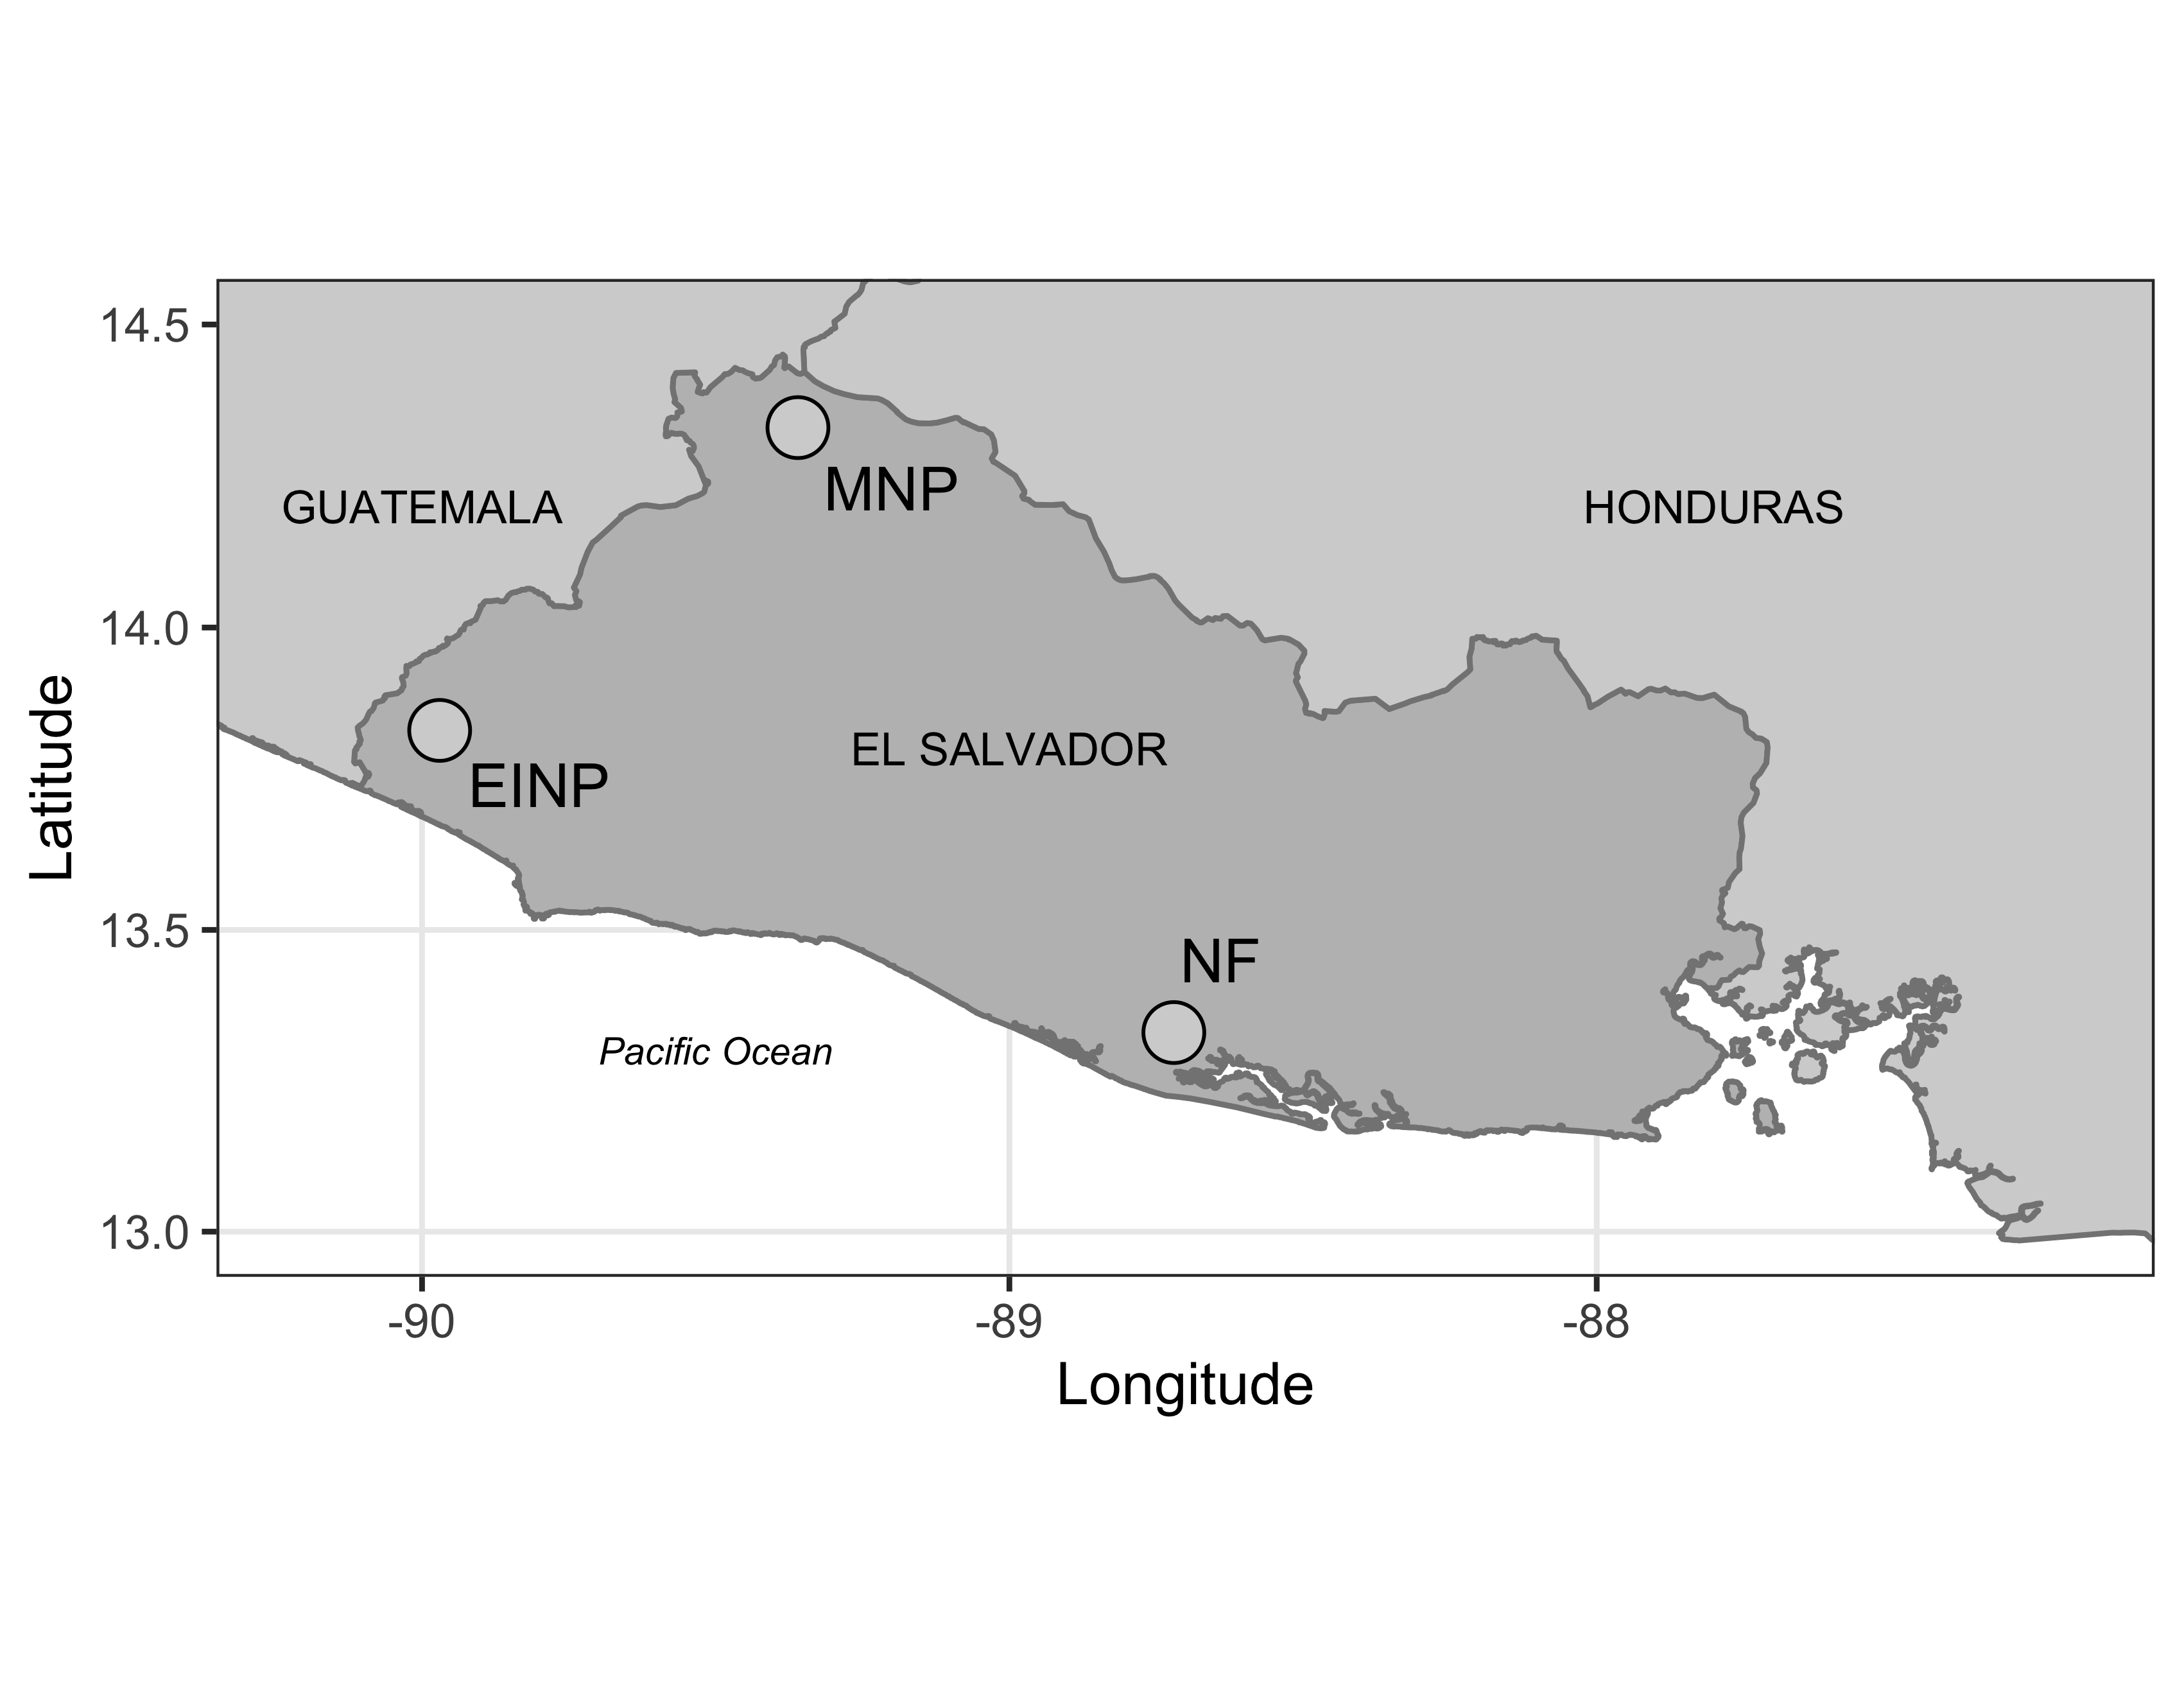
\includegraphics{../output/figures/map-1.png}
\caption{1XX. Map of El Salvador. Owl surveys were conducted from 2003
to 2013 in three different protected areas within El Salvador: El
Imposible National Park (EINP), Montecristo National Park (MNP) and
Nancuchiname Forest (NF). \label{map}}
\end{figure}

\begin{figure}
\centering
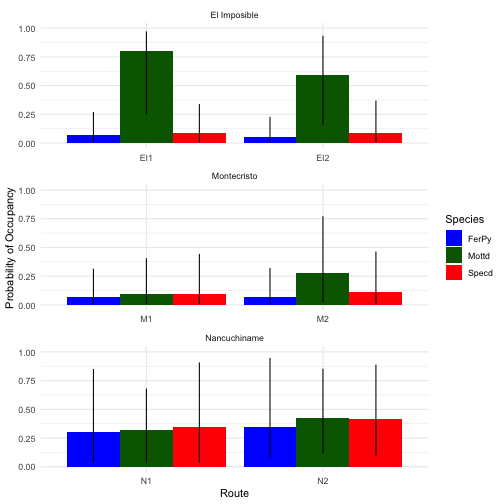
\includegraphics{../output/figures/psi_means-1.png}
\caption{2XX. Probability of occupancy (\(\psi_{t,h}\)) summarized by
route for Ferruginous Pygmy-owl (FEPO), Mottled Owl (MOOW), and
Spectacled Owl (SPEO). Owl surveys were conducted from 2003 to 2013 in
three different protected areas within El Salvador: El Imposible
National Park (EI-1 and EI-2), Montecristo National Park (M-1 and M-2)
and Nancuchiname Forest (N-1 and N-2). Posteriors were summarized with
median \(\pm\) 90\% credible intervals. \label{psi_means}}
\end{figure}

\begin{figure}
\centering
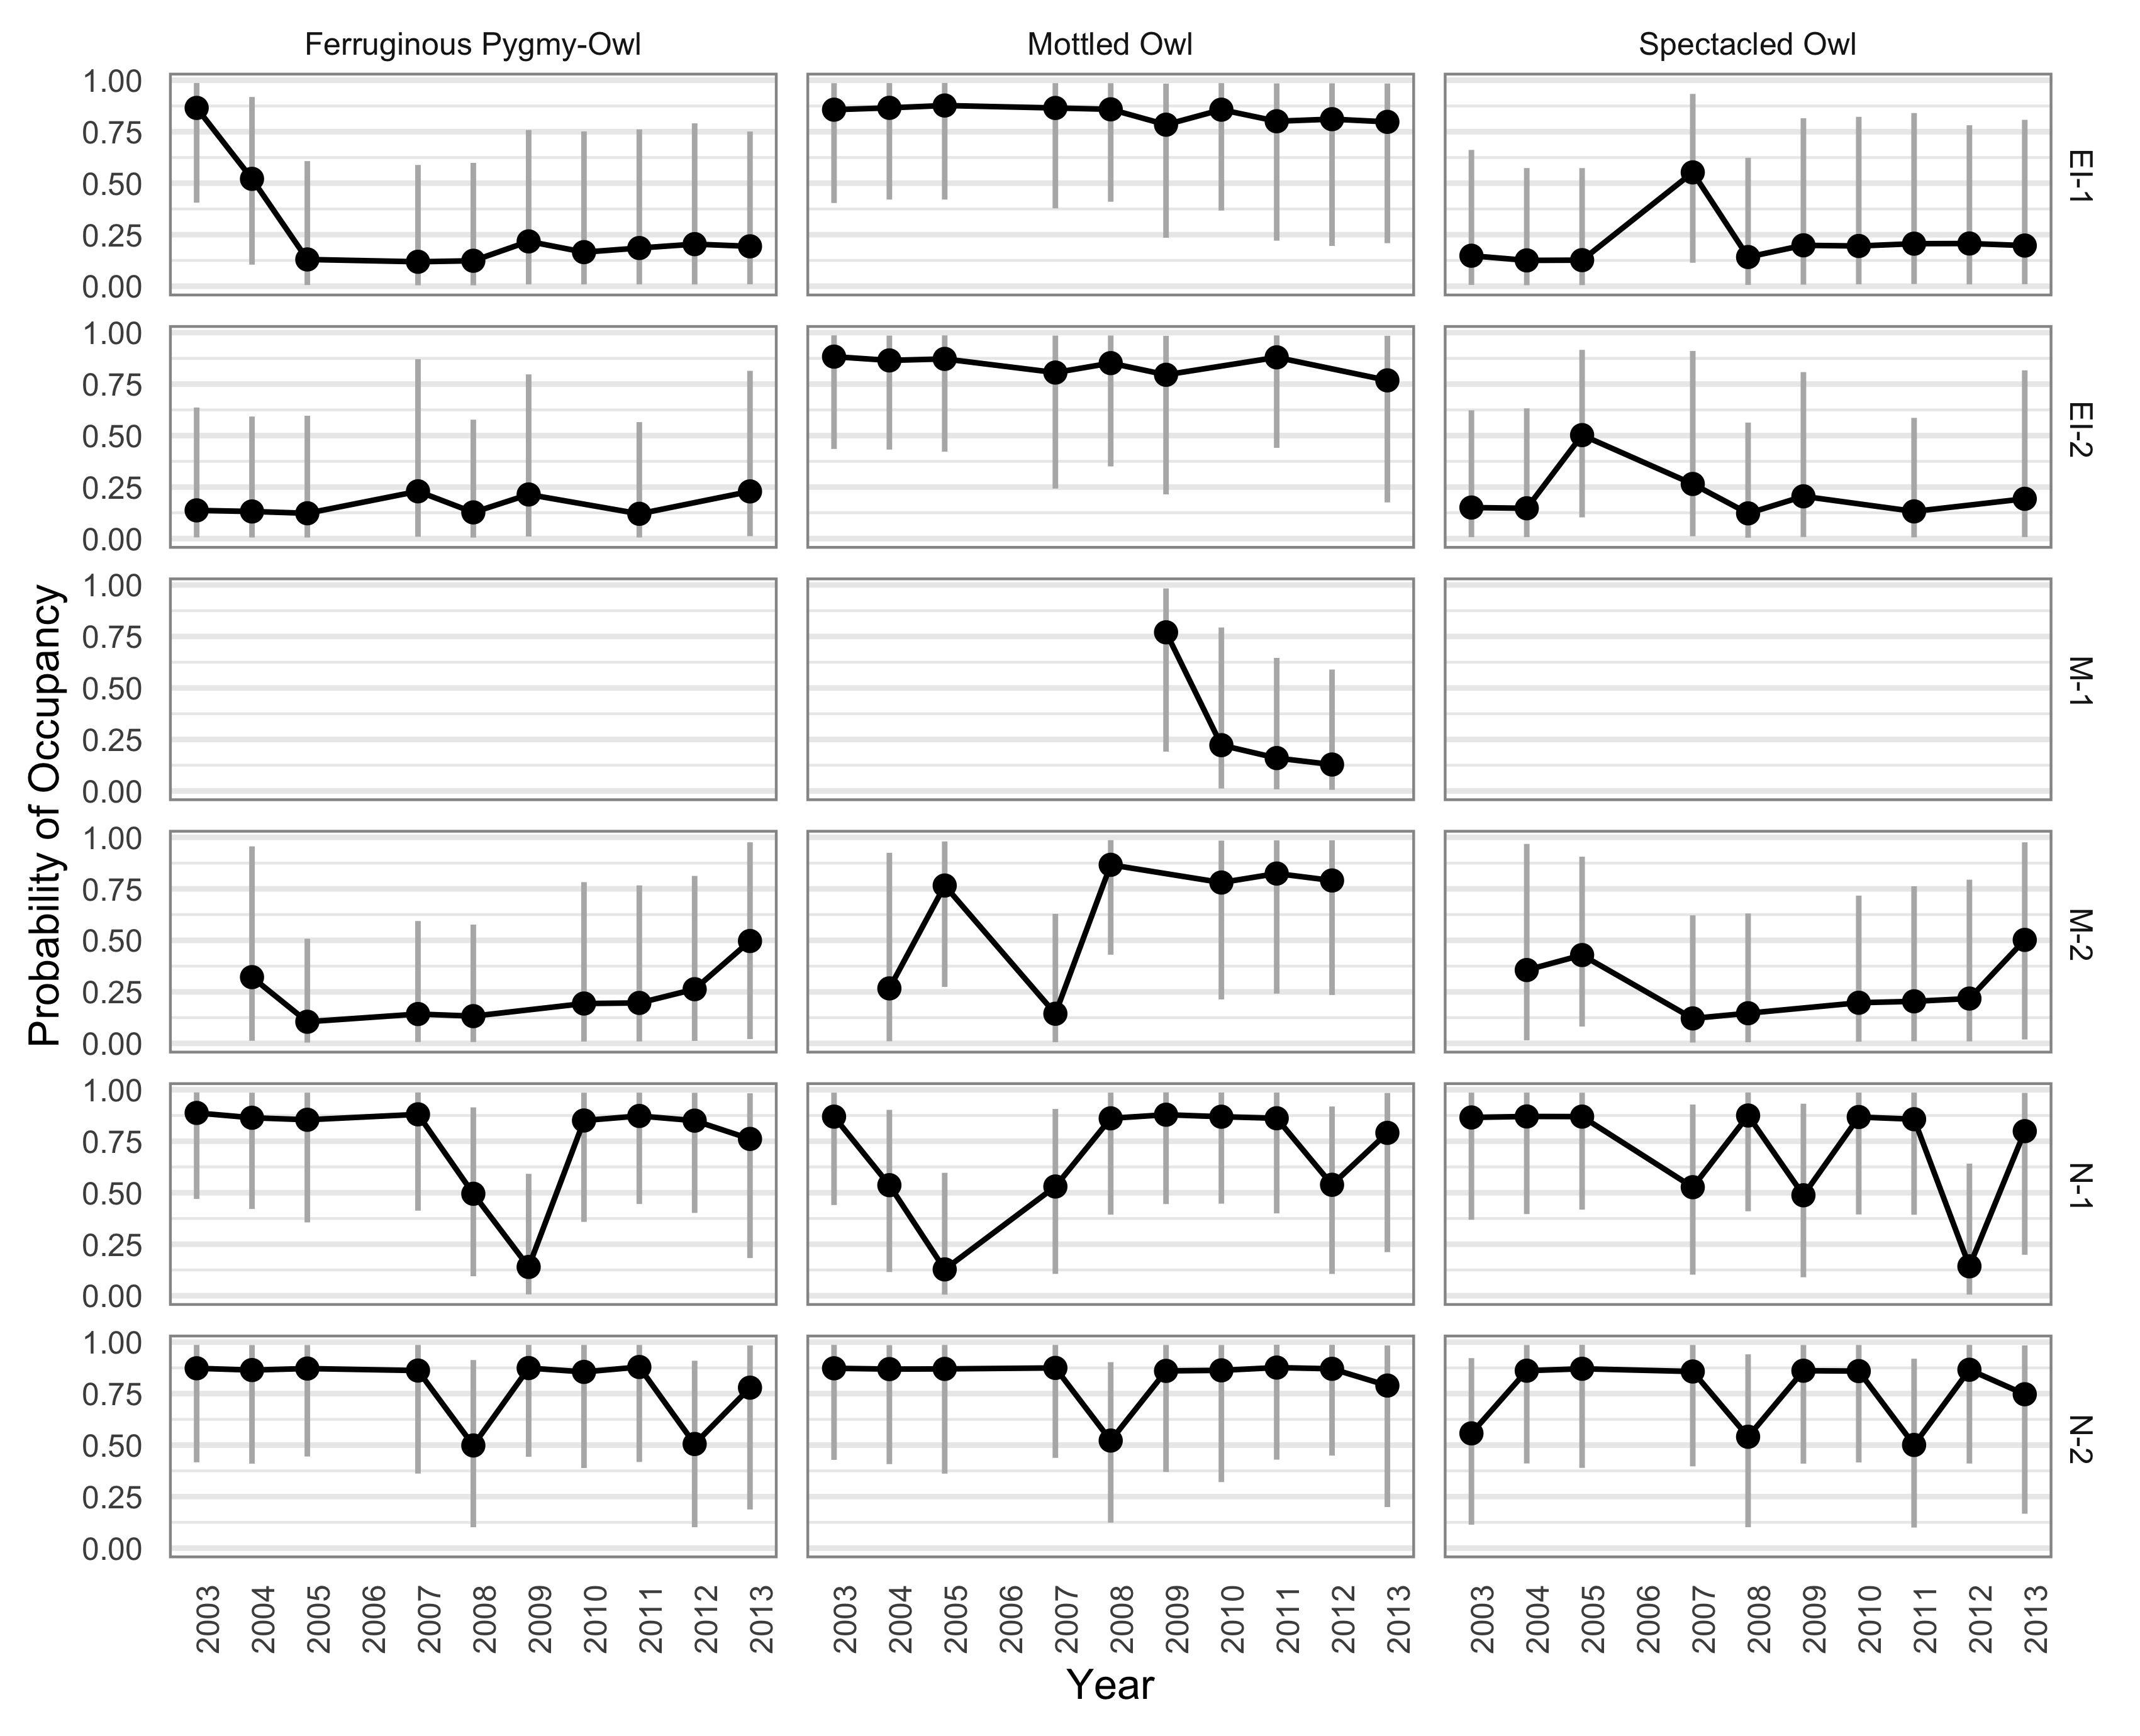
\includegraphics{../output/figures/psi_byYr-1.png}
\caption{3XX. Probability of occupancy by route and year for Ferruginous
Pygmy-owl (FEPO), Mottled Owl (MOOW), and Spectacled Owl (SPEO). Owl
surveys were conducted from 2003 to 2013 in three different protected
areas within El Salvador: El Imposible National Park (EI-1 and EI-2),
Montecristo National Park (M-1 and M-2) and Nancuchiname Forest (N-1 and
N-2). Posteriors were summarized with median \(\pm\) 90\% credible
intervals. \label{figure2}}
\end{figure}

\begin{figure}
\centering
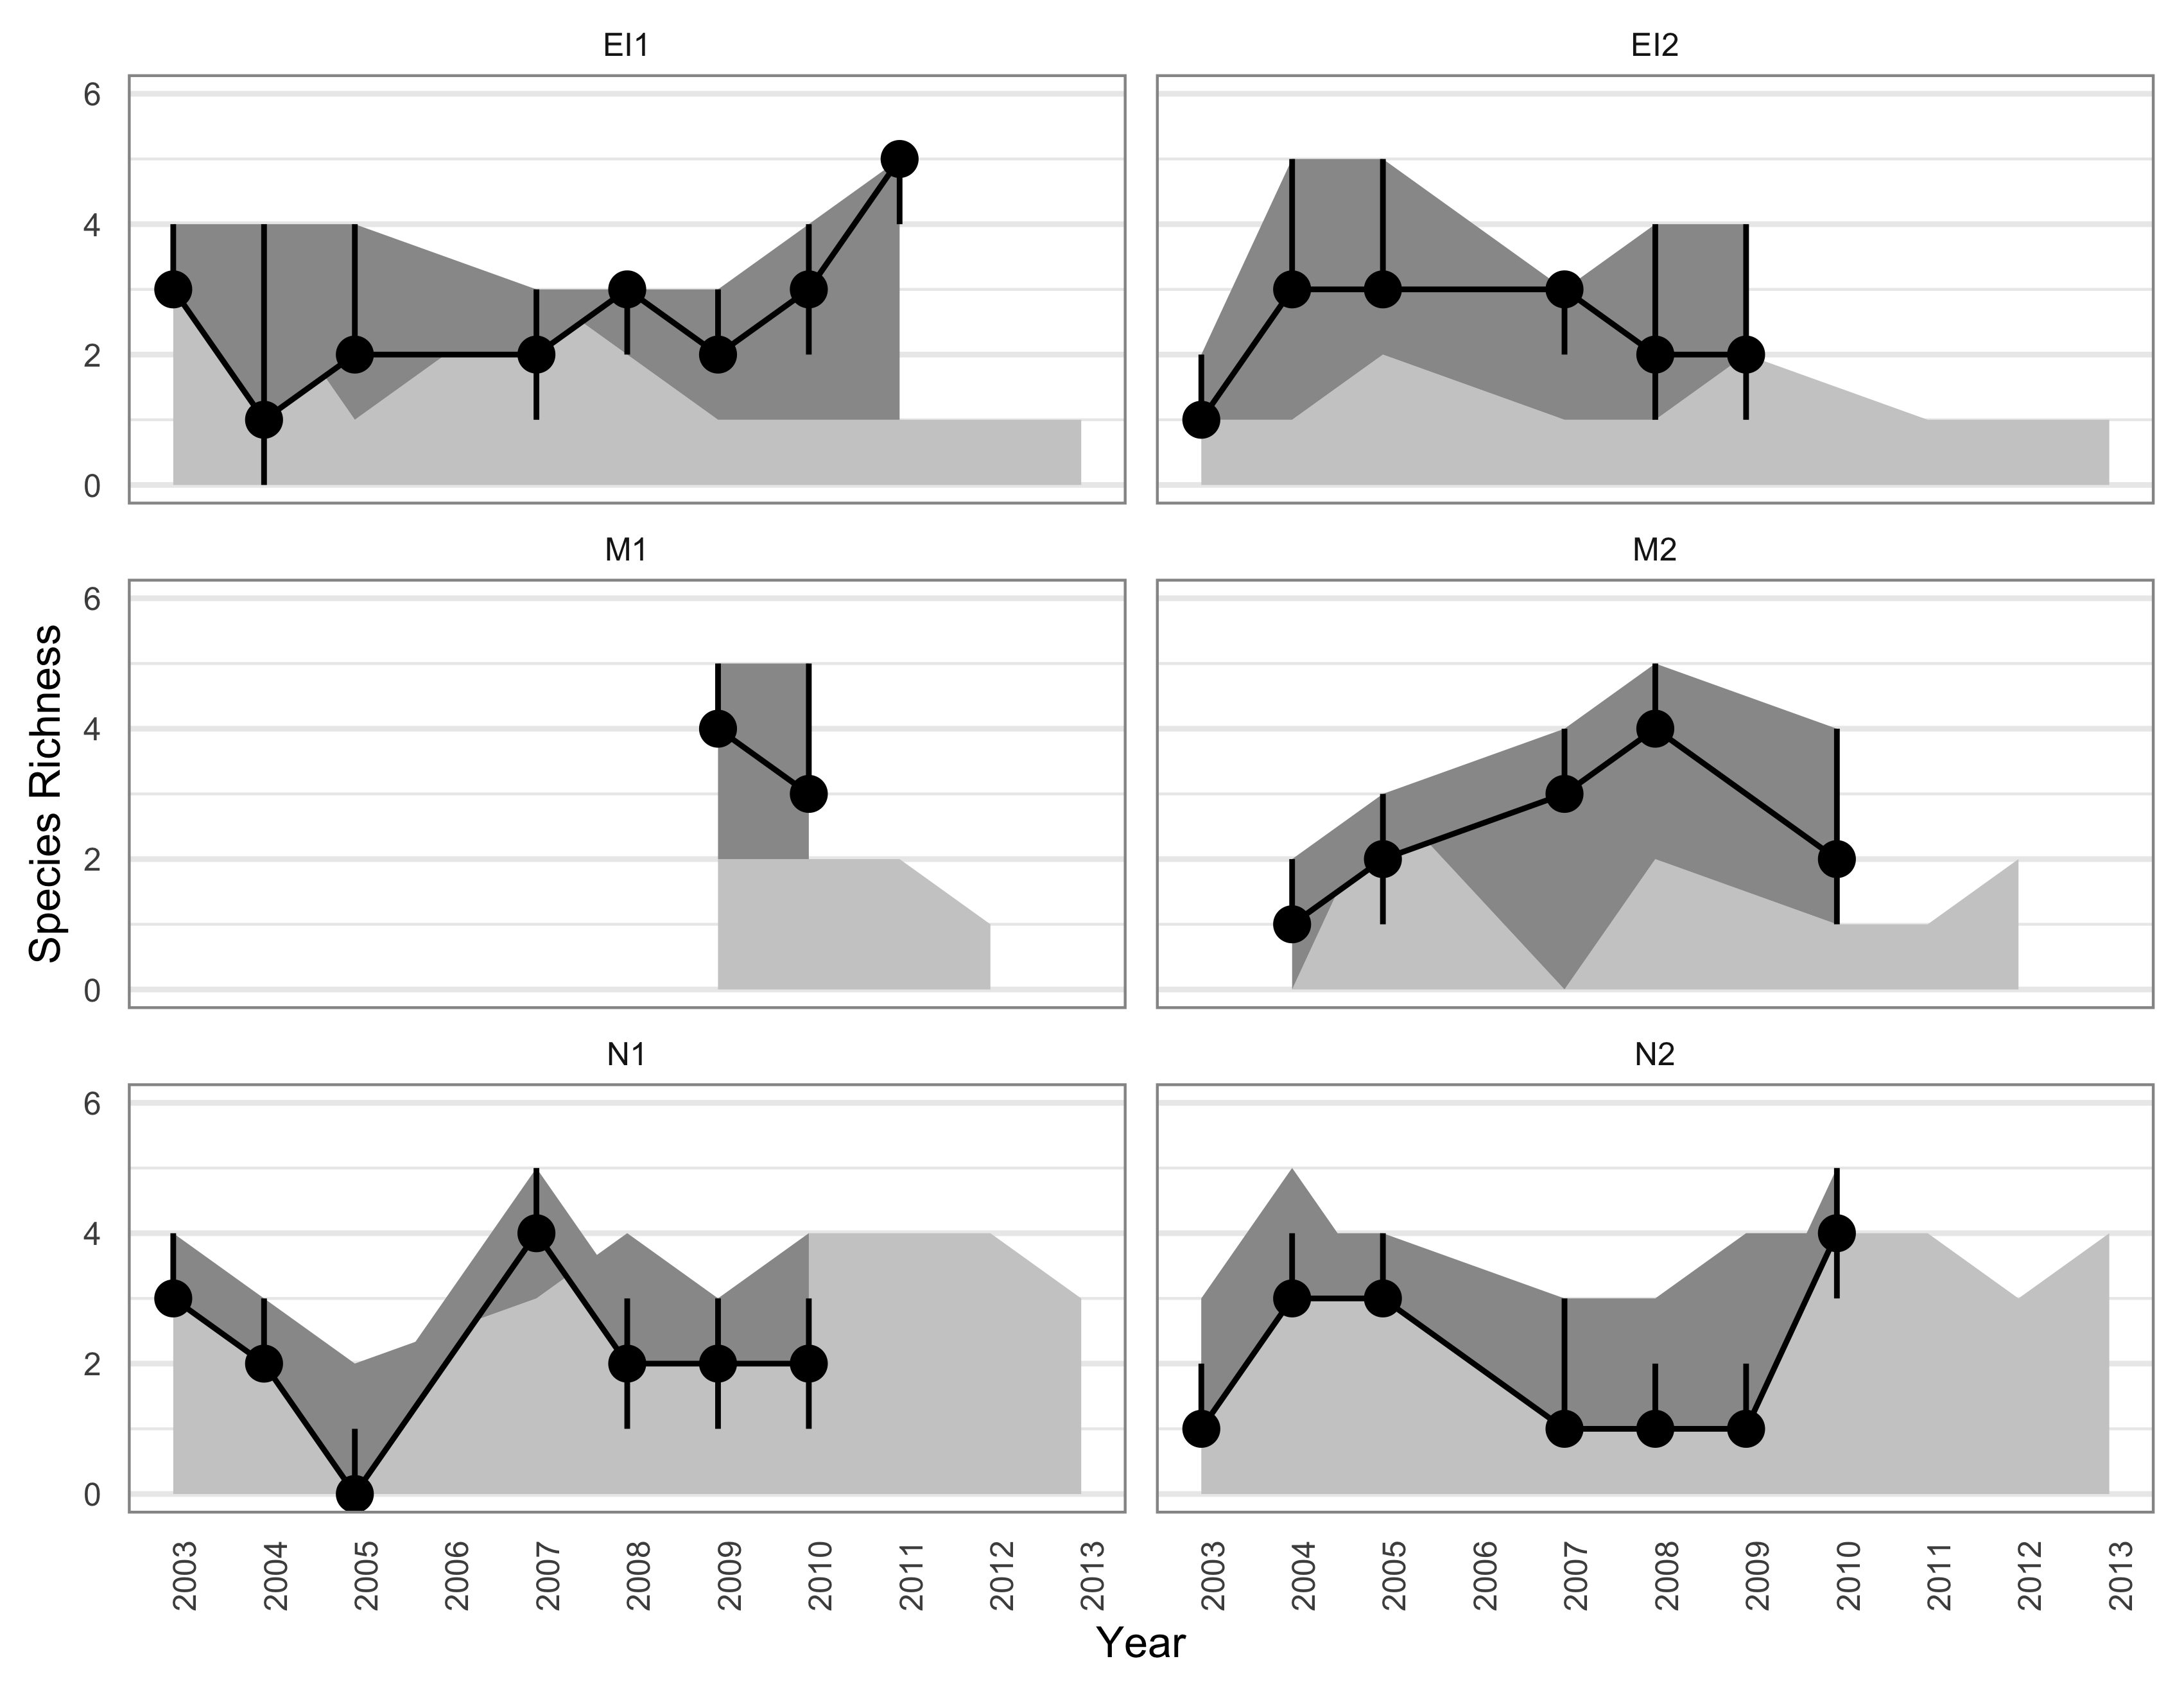
\includegraphics{../output/figures/richness_byRtYr-1.png}
\caption{4XX. Species richness (Richness\emph{) by route and year. Owl
surveys were conducted from 2003 to 2013 in three different protected
areas within El Salvador: El Imposible National Park (EI-1 and EI-2),
Montecristo National Park (M-1 and M-2) and Nancuchiname Forest (N-1 and
N-2). Posteriors of Richness} were summarized with median (black dot)
\(\pm\) 90\% credible intervals (dark grey shading and vertical black
lines). The number of owl species detected at each route and year was
indicated with the light grey area. \label{figure5}}
\end{figure}

\begin{figure}
\centering
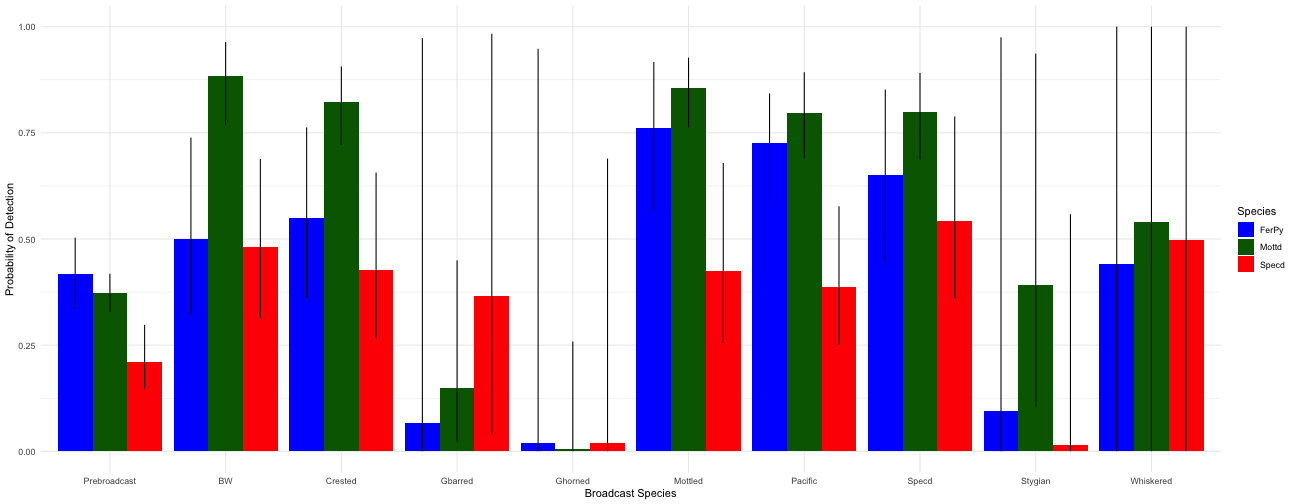
\includegraphics{../output/figures/p_detection-1.png}
\caption{5XX. The probabiliity of detecting owls during spontaneous
surveys (i.e., pre-broadcast) and after broadcast, depending on the
species of owl used for broadcast vocalization. These logistic
regression coefficients were evaluated from the richness model, which
combined all detected species (All Species) and the single-species
occupancy models for Ferruginous Pygmy-owls (FEPO), Mottled Owls (MOOW),
and Spectacled Owls (SPEO). Owl surveys were conducted from 2003 to 2013
in three different protected areas within El Salvador. Posteriors were
summarized with median \(\pm\) 90\% credible intervals. The
pre-broadcase effect size's credible intervals are represented with two
grey horizontal lines on each graph \label{figure6}}
\end{figure}

\hypertarget{references}{%
\section*{References}\label{references}}
\addcontentsline{toc}{section}{References}

\hypertarget{refs}{}
\leavevmode\hypertarget{ref-Andersen:2007}{}%
Andersen, D. E. 2007. Survey techniques. Pages 89--100 \emph{in} D. M.
Bird and K. L. Bildstein, editors. Raptor research and management
techniques. Hancock House Publishers, Blaine, WA USA.

\leavevmode\hypertarget{ref-Alvarez:2003}{}%
Álvarez, J. M., and O. Komar. 2003. El parque nacional el imposible y su
vida silvestre. Salva Natura y Ministerio de Medio Ambiente y Recursos
Naturales.

\leavevmode\hypertarget{ref-Baumgardt:2019}{}%
Baumgardt, J. A., M. L. Morrison, L. A. Brennan, and T. A. Campbell.
2019. Effects of broadcasting calls on detection probability in
occupancy analyses of multiple raptor species. Western North American
Naturalist 79:185--194.

\leavevmode\hypertarget{ref-Borges:2004}{}%
Borges, S. H., L. M. Henriques, and A. Carvalhaes. 2004. Density and
habitat use by owls in two Amazonian forest types. Journal of Field
Ornithology 75:176--182.

\leavevmode\hypertarget{ref-Broms:2016}{}%
Broms, K. M., M. B. Hooten, and R. M. Fitzpatrick. 2016. Model selection
and assessment for multi-species occupancy models. Ecology
97:1759--1770.

\leavevmode\hypertarget{ref-Buechley:2019}{}%
Buechley, E. R., A. Santangeli, M. Girardello, M. H. C. Neate-Clegg, D.
Oleyar, C. J. W. McClure, and Ç. H. Şekercioğlu. 2019. Global raptor
research and conservation priorities: Tropical raptors fall prey to
knowledge gaps. Diversity and Distributions 25:856--869.

\leavevmode\hypertarget{ref-Campioni:2013}{}%
Campioni, L., J. H. Sarasola, M. Santillán, and M. M. Reyes. 2013.
Breeding season habitat selection by Ferruginous Pygmy Owls
\emph{Glaucidium brasilianum} in central Argentina. Bird Study
60:35--43.

\leavevmode\hypertarget{ref-CIA:2020}{}%
Central Intelligence Agency. 2020. The world factbook.
www.cia.gov/the-world-factbook.

\leavevmode\hypertarget{ref-Clark:1978}{}%
Clark, R. J., D. G. Smith, and L. H. Kelso. 1978. Working bibliography
of owls of the world. National Wildlife Federation Scientific and
Technical Series.

\leavevmode\hypertarget{ref-Corlett:2012}{}%
Corlett, R. T. 2012. Climate change in the tropics: The end of the world
as we know it? Biological Conservation 151:22--25.

\leavevmode\hypertarget{ref-Dickey:1938}{}%
Dickey, D. R., and A. J. van Rossem. 1938. The birds of El Salvador.
Field Museum of Natural History.

\leavevmode\hypertarget{ref-Enriquez:1997}{}%
Enrı́quez, P. L., and J. L. R. Salazar. 1997. Intra-and interspecific
calling in a tropical owl community. \emph{in} In: Duncan, james r.;
johnson, david h.; nicholls, thomas h., eds. Biology and conservation of
owls of the northern hemisphere: 2nd international symposium. Gen. Tech.
Rep. NC-190. St. Paul, mn: US dept. Of agriculture, forest service,
north central forest experiment station. 525-532.

\leavevmode\hypertarget{ref-Enriquez:2001}{}%
Enrı́quez, P., and J. Rangel-Salazar. 2001. Owl occurrence and calling
behavior in a tropical rain forest. Journal of Raptor Research
35:107--114.

\leavevmode\hypertarget{ref-Enriquez:2006}{}%
Enríquez, P. L., D. H. Johnson, and J. L. Rangel-Salazar. 2006.
Taxonomy, distribution and conservation of owls in the Neotropics: A
review. Pages 254--307 \emph{in} R. Rodríguez-Estrella, editor. Current
Raptor Studies in México. Comisión Nacional para el Conocimiento y Uso
de la Biodiversidad.

\leavevmode\hypertarget{ref-Enriquez-Rocha:1993}{}%
Enríquez-Rocha, P., J. L. Rangel-Salazar, and D. W. Holt. 1993. Presence
and distribution of Mexican owls: a review. Journal of Raptor Research
27:154--160.

\leavevmode\hypertarget{ref-Esclarski:2014}{}%
Esclarski, P., and R. Cintra. 2014. Effects of terra firm-forest
structure on habitat use by owls (Aves: Strigiformes) in central
Brazilian Amazonia. Ornitological Neotropical 25:433--458.

\leavevmode\hypertarget{ref-Flesch:2007}{}%
Flesch, A. D., and R. J. Steidl. 2007. Detectability and response rates
of Ferruginous Pygmy-Owls. The Journal of Wildlife Management
71:981--990.

\leavevmode\hypertarget{ref-Fuller:1987}{}%
Fuller, M. R., and J. A. Mosher. 1987. Raptor survey techniques.
\emph{in} Raptor research techniques manual. US Fish and Wildlife
Service.

\leavevmode\hypertarget{ref-Gelman:2008}{}%
Gelman, A., A. Jakulin, M. G. Pittau, and Y.-S. Su. 2008. A weakly
informative default prior distribution for logistic and other regression
models. The Annals of Applied Statistics 2:1360--1383.

\leavevmode\hypertarget{ref-Gerhardt:1989}{}%
Gerhardt, R. P. 1989. Response of the Mottled Owl (\emph{Ciccaba
virgata}) to broadcast of conspecific call. \emph{in} W. A. Burnham, J.
P. Jenny, and C. W. Turley, editors. Maya project: Use of raptors as
environmental indices for design and management of protected areas and
for building local capacity for conservation in latin america. The
Peregrine Fund, Inc., World Center for Birds of Prey.

\leavevmode\hypertarget{ref-Gonzalez:2017}{}%
Gonzalez, R., R. Pineda, and L. Pineda. 2017. Photographic documentation
of Fulvous Owl (\emph{Strix fulvescens} in Montecristo National Park, El
Salvador. Spizaetus Neotropical Raptor Network Newsletter. 24:16--21.

\leavevmode\hypertarget{ref-Guillera-Arroita:2019}{}%
Guillera-Arroita, G., M. Kéry, and J. J. Lohoz-Monfort. 2019. Inferring
species richness using multispecies occupancy modeling: Estimation
performance and interpretation. Ecology and Evolution 9:780--792.

\leavevmode\hypertarget{ref-Johnsgard:1988}{}%
Johnsgard, P. A. 1988. North american owls: Biology and natural history.
Yale University Press, New Haven, CT.

\leavevmode\hypertarget{ref-Komar:2002}{}%
Komar, O. 2002. Priority conservation areas for birds in El Salvador.
Animal Conservation 5:173--183.

\leavevmode\hypertarget{ref-Komar:2010}{}%
Komar, O. 2010. Research stewardship strategy for Montecristo National
Park, El Salvador. Technical report, USAID.

\leavevmode\hypertarget{ref-Konig:1999}{}%
König, C., and F. Weick. 1999. Owls: A guide to owls of the world. Yale
University Press, New Haven, CT.

\leavevmode\hypertarget{ref-Marin-Gomez:2017}{}%
Marín-Gómez, O. H., Y. Toro-López, M. M. López-García, J. I. Garzón
Zuluaga, and D. M. Santa-Aristizabal. 2017. First records of the
Spectacled Owl (\emph{Pulsatrix perspicillata}) in urban areas, with
notes on reproduction. North-Western Journal of Zoology 13:2.

\leavevmode\hypertarget{ref-Mikkola:2012}{}%
Mikkola, H. 2012. Owls of the world-a photographic guide. Firefly Books,
Buffalo, New York, NY, USA.

\leavevmode\hypertarget{ref-MARN:2010}{}%
Ministerio de Medio Ambiente y Recursos Naturales. 2010. Guía de Aves
Parque Nacional Montecristo. Guías de la Biodiversidad del Parque
Nacíonal Montecristo. San Salvador, El Salvador.

\leavevmode\hypertarget{ref-MARN:2015b}{}%
Ministerio de Medio Ambiente y Recursos Naturales. 2015a. La guía de
aves del Parque Nacíonal Montecristo. Parte de la serie de guías de la
biodiversidad del Parque Nacíonal Montecristo. San Salvador, El
Salvador.

\leavevmode\hypertarget{ref-MARN:2015}{}%
Ministerio de Medio Ambiente y Recursos Naturales. 2015b. Acuerdo No.~74
Listado oficial de especíes de vida silvestre amenazadas o en peligro de
extinción. San Salvador, El Salvador.

\leavevmode\hypertarget{ref-Myers:2000}{}%
Myers, N., and R. A. Mittermeier. 2000. Biodiversity hotspots for
conservation priorities. Nature 403:853.

\leavevmode\hypertarget{ref-Orihuela-Torres:2018}{}%
Orihuela-Torres, A., L. Ordóñez-Delgado, A. Verdezoto-Celi, and J.
Brito. 2018. Diet of Spectacled Owl (\emph{Pulsatrix perspicillata}) in
Zapotillo, southwestern Ecuador. Revista Brasileira de Ornitologia
26:52--56.

\leavevmode\hypertarget{ref-Perez-Leon:2017}{}%
Pérez-Léon, R., I. Vega, and N. Herrera. 2017. The owls of El Salvador.
Pages 397--418 \emph{in} P. L. Enríquez, editor. Neotropical owls:
Diversity and Conservation. Springer International Publishing AG, Cham,
Switzerland.

\leavevmode\hypertarget{ref-Plummer:2013}{}%
Plummer, M. 2013. JAGS Version 3.4.0 user manual.

\leavevmode\hypertarget{ref-Rangel-Salazar:2017}{}%
Rangel-Salazar, J. L., and P. L. Enríquez. 2017. Introduction: The birds
in the neotropical region. Pages 1--6 \emph{in} Neotropical owls.
Springer.

\leavevmode\hypertarget{ref-R:2014}{}%
R Development Core Team. 2014. R: A Language and Environment for
Statistical Computing. R Foundation for Statistical Computing, Vienna,
Austria.

\leavevmode\hypertarget{ref-Royle:2007}{}%
Royle, J. A. 2007. Analysis of multinomial models with unknown index
using data augmentation. Journal of Computational and Graphical
Statistics 16:67--85.

\leavevmode\hypertarget{ref-Sarasola:2014}{}%
Sarasola, J. H., and M. Á. Santillán. 2014. Spatial and temporal
variation in the feeding ecology of ferruginous pygmy-owls
(\emph{Glaucidium brasilianum}) in semiarid forests of central
Argentina. Journal of Arid Environments 109:39--43.

\leavevmode\hypertarget{ref-Silva:2016}{}%
Silva, R. O. 2016. Country coffee profile: El Salvador. Technical
report, International Coffee Organization.

\leavevmode\hypertarget{ref-Takats:2001}{}%
Takats, D. L., C. M. Francis, G. L. Holroyd, J. R. Duncan, K. M. Mazur,
R. J. Cannings, W. Harris, and D. Holt. 2001. Guidelines for nocturnal
owl monitoring in North America. Beaverhill Bird Observatory and Bird
Studies Canada.

\leavevmode\hypertarget{ref-Terry:2005}{}%
Terry, A. M., T. M. Peake, and P. K. McGregor. 2005. The role of vocal
individuality in conservation. Frontiers in Zoology 2:10.

\leavevmode\hypertarget{ref-USFWS:1995}{}%
United States Fish and Wildlife Service. 1995. Recovery plan for the
Mexican Spotted Owl. Technical report, United States Department of the
Interior.

\leavevmode\hypertarget{ref-Vallely:2018}{}%
Vallely, A. C., and D. Dyer. 2018. Birds Of Central America: BELIZE,
GUATEMALA, HONDURAS, EL SALVADOR, NICARAGUA, COSTA RICA, and PANAMA.
Princeton University Press, Princeton, NJ, USA.

\leavevmode\hypertarget{ref-Wan:2018}{}%
Wan, H. Y., J. L. Ganey, C. D. Vojta, and S. A. Cushman. 2018. Managing
emerging threats to spotted owls. The Journal of Wildlife Management
82:682--697.

\leavevmode\hypertarget{ref-West:1988}{}%
West, J. N. 1988. Raptors of El Imposible Forest, El Salvador. Masters
thesis, Central Washington University, Ellensburg, WA.

\leavevmode\hypertarget{ref-White:2013}{}%
White, A. M., E. F. Zipkin, P. N. Manley, and M. D. Schlesinger. 2013.
Conservation of avian diversity in the Sierra Nevada: Moving beyond a
single-species management focus. PLoS ONE 8:e63088.

\leavevmode\hypertarget{ref-Zepeda:1995}{}%
Zepeda, L. 1995. Plan de manejo del área natural silvestre Nancuchiname.
Anexo 4 - listado preliminar de las aves del área, San Salvador, El
Salvador.

\end{document}
